\documentclass[a4paper,12pt]{article}

%%% Работа с русским языком

\usepackage{cmap}					% поиск в PDF
\usepackage{mathtext} 				% русские буквы в формулах
\usepackage[T2A]{fontenc}			% кодировка
\usepackage[utf8]{inputenc}			% кодировка исходного текста
\usepackage[english,russian]{babel}	% локализация и переносы
\usepackage{indentfirst}            % красная строка в первом абзаце
\usepackage[unicode]{hyperref}
\usepackage{epigraph}
\usepackage{textcomp}
\usepackage{marvosym}
\usepackage{fontawesome}
\frenchspacing                      % равные пробелы между словами и предложениями

%%% Дополнительная работа с математикой
\usepackage{amsmath,amsfonts,amssymb,amsthm,mathtools} % пакеты AMS
\usepackage{bbm} % Blackboard bold для цифр
\usepackage{icomma}                                    % "Умная" запятая

\renewcommand{\phi}{\ensuremath{\varphi}}
\renewcommand{\kappa}{\ensuremath{\varkappa}}
\renewcommand{\le}{\ensuremath{\leqslant}}
\renewcommand{\leq}{\ensuremath{\leqslant}}
\renewcommand{\ge}{\ensuremath{\geqslant}}
\renewcommand{\geq}{\ensuremath{\geqslant}}
\renewcommand{\emptyset}{\ensuremath{\varnothing}}

\newcommand{\cl}{\text{cl }}
\newcommand{\setint}{\text{int }}
\newcommand\independent{\protect\mathpalette{\protect\independenT}{\perp}}
\def\independenT#1#2{\mathrel{\rlap{$#1#2$}\mkern2mu{#1#2}}}

\theoremstyle{plain}
\newtheorem{theorem}{Теорема}[subsection]
\newtheorem{lemma}{Лемма}[subsection]
\newtheorem{proposition}{Утверждение}[subsection]
\newtheorem*{corollary}{Следствие}
\newtheorem*{exercise}{Упражнение}

\theoremstyle{definition}
\newtheorem{definition}{Определение}[subsection]
\newtheorem*{note}{Замечание}
\newtheorem*{reminder}{Напоминание}
\newtheorem*{example}{Пример}
\newtheorem*{tasks}{Вопросы и задачи}

\theoremstyle{remark}
\newtheorem*{solution}{Решение}

%%% Оформление страницы
\usepackage{extsizes}     % Возможность сделать 14-й шрифт
\usepackage{geometry}     % Простой способ задавать поля
\usepackage{setspace}     % Интерлиньяж
\usepackage{enumitem}     % Настройка окружений itemize и enumerate
\usepackage{epigraph}     % Эпиграф
\setlist{leftmargin=25pt} % Отступы в itemize и enumerate

\geometry{top=25mm}    % Поля сверху страницы
\geometry{bottom=30mm} % Поля снизу страницы
\geometry{left=20mm}   % Поля слева страницы
\geometry{right=20mm}  % Поля справа страницы

\title{Экзамен по формальным языкам}

\begin{document}
\tableofcontents
\newpage

\section{Автоматы и регулярные выражение}
\subsection{Про НКА}
\subsubsection*{Недетерминированные конечные автоматы.}
\begin{definition}
	\textbf{Алфавит} - непустое конечное множество, элементы которого называются символами. Обозначение: $\Sigma$.
\end{definition}

\begin{note} Дополнительные обозначения.

	\begin{itemize}
		\item $\Sigma^*$ -- множество слов, состоящее из всех символов алфавита $\Sigma$.
		\item \textbf{Формальный язык} $L \subset \Sigma^*$.
		\item Пустое слово $\varepsilon \subset \Sigma^*$.
	\end{itemize}
\end{note}

\begin{definition}
	\textbf{Конкатенацией} языков $L_1$ и $L_2$ называется язык:
	\[
		L_1L_2 := L_1\cdot L_2 := \{uv \:|\: u \in L_1,\, v \in L_2\}
	\]
\end{definition}

\begin{definition}
	\textbf{Недетерминированный конечный автомат} -- кортеж $M = \langle Q,\,\Sigma,\, \Delta,\, q_0,\, F \rangle$, где:
	\begin{itemize}
		\item $Q$ -- множество состояний, $|Q| < +\infty$.
		\item $\Sigma$ -- алфавит.
		\item $\Delta \subset Q \times \Sigma^* \times Q$ -- множество переходов.
		\item $q_0 \in Q$ -- стартовое состояние.
		\item $F \subset Q$ -- множество завершающих состояний.
	\end{itemize}
\end{definition}

\begin{definition}
	\textbf{Конфигурация} в автомате $M = \langle Q,\,\Sigma,\, \Delta,\, q_0,\, F \rangle$ -- элемент $\langle q,\, w\rangle \in Q \times \Sigma^*$.
\end{definition}

\begin{definition}
	$\vdash$ -- наименьшее рефлексивное транзитивное отношение над $Q \times \Sigma^*$, такое, что:
	\[
		\forall w \in \Sigma^*:\: (\langle q_1,\,w\rangle \to q_2) \in \Delta \Rightarrow \forall u \in \Sigma^*:\: \langle q_1,\,wu\rangle \vdash \langle q_2,\,u\rangle
	\]
\end{definition}

\subsubsection*{Автоматные языки: примеры автоматных языков}
\begin{definition}
	Для автомата $M = \langle Q,\,\Sigma,\, \Delta,\, q_0,\, F \rangle$ языком, задаваемым автоматом, называется:
	\[
		L(M) = \{w \in \Sigma^* \:|\: \exists q \in F :\: \langle q_0,\, w\rangle \vdash \langle q,\, \varepsilon\rangle\}
	\]
\end{definition}

\begin{definition}
	Язык $L$ называется \textbf{автоматным}, если существует такой НКА $M$, что $L = L(M)$
\end{definition}

\begin{example}
	Постройте какой-нибудь простой автомат и докажите включение в обе стороны.
\end{example}

\subsubsection*{Различные варианты определений (упрощения НКА)}
\begin{proposition}
	В определении автомата можно считать: $M = \langle Q,\,\Sigma,\, \Delta,\, q_0,\, F \rangle$, где $|F| = 1$.
\end{proposition}

\begin{proof}
	Пусть $M = \langle Q,\,\Sigma,\, \Delta,\, q_0,\, F \rangle$ -- исходный НКА.

	Построим $M' = \langle Q \cup \{q_f\},\,\Sigma,\, \Delta',\, q_0,\, \{q_f\} \rangle$, где:
	\[
		\Delta' = \Delta \cup \{\langle q,\, \varepsilon\rangle \to q_f \:|\: q \in F\}
	\]
	Покажем, что $L(M) = L(M')$.

	В начале покажем, что $L(M) \subset L(M')$:
	\begin{itemize}
		\item $w \in L(M) \Rightarrow \exists q \in F:\: \langle q_0,\, w\rangle \vdash \langle q,\, \varepsilon\rangle$
		\item $(\langle q,\, \varepsilon\rangle \to q_f) \in \Delta' \Rightarrow \langle q,\, \varepsilon\rangle \vdash_{M'} \langle q_f,\, \varepsilon\rangle$
		\item Значит $\langle q_0,\, w\rangle \vdash_{M'} \langle q,\, \varepsilon\rangle \vdash_{M'} \langle q_f,\, \varepsilon\rangle \Rightarrow w \in L(M')$
	\end{itemize}
	Теперь докажем обратное включение $L(M') \subset L(M)$:
	\begin{itemize}
		\item $w \in L(M') \Rightarrow \langle q_0,\, w\rangle \vdash_{M'} \langle q_f,\, \varepsilon\rangle$
		\item Рассмотрим цепь $\langle q_0,\, w\rangle \vdash_{M'} \langle q,\, u\rangle \vdash_{M',\, 1} \langle q_f,\, \varepsilon\rangle$
		\item Тогда $u = \varepsilon$, а $q \in F$ из того, как мы определили $\Delta'$ (других переходов в $q_f$ не существует).
		\item Получили $\langle q_0,\, w\rangle \to q \Rightarrow w \in L(M)$.
	\end{itemize}
\end{proof}

\begin{proposition}
	Для любого автоматного языка $L$ существует НКА $M = \langle Q,\,\Sigma,\, \Delta,\, q_0,\, F \rangle$, такой что $L = L(M)$ и:
	\[
		\forall (\langle q_1,\, w\rangle \to q_2) \in \Delta :\: |w| \leq 1
	\]
\end{proposition}

\begin{proof}
	Разобьём все $n$-буквенные переходы на $n$ однобуквенных переходов.
\end{proof}

\begin{proposition}
	Для любого НКА $M = \langle Q,\,\Sigma,\, \Delta,\, q_0,\, F \rangle$ существует НКА $M' = \langle Q,\,\Sigma,\, \Delta',\, q_0,\, F' \rangle$, такой, что $L(M) = L(M')$ и:
	\[
		\forall (\langle q_1,\, w\rangle \to q_2) \in \Delta' :\: |w| = 1
	\]
\end{proposition}

\begin{proof}
	Обозначим $\Delta(q,\, w) = \{q' \:|\: \langle q,\, w\rangle \vdash \langle q',\, \varepsilon\rangle\}$, то есть вершины, достижимые по слову $w$.

	Тогда новое множество переходов определим, как:
	\[
		\Delta' = \{\langle q_1,\, a\rangle \to q_2 \:|\: \exists q_3 \in \Delta(q_1,\,\varepsilon) :\: (\langle q_3,\, a\rangle \to q_2) \in \Delta\}
	\]
	Новым же множеством завершающих состояний будет:
	\[
		F' = \{q' \:|\: \Delta(q',\, \varepsilon) \cap F \neq \emptyset\}
	\]
	Покажем же теперь, что $L(M) = L(M')$.

	В начале докажем $L(M) \subset L(M')$. Тогда $\exists q \in F :\: \langle q_0,\, w\rangle \vdash \langle q,\, \varepsilon\rangle$. Б.О.О. будем считать, что $w = w_1w_2,\, w_i \in \Sigma$. Тогда существует цепь:
	\begin{itemize}
		\item $\langle q_0,\, w_1w_2\rangle \vdash_M \langle q_1',\, w_1w_2\rangle$ -- перешли по цепочке эпсилонов, где $q_1'$ альтер-эго $q_3$ из определения $\Delta'$.
		\item $\langle q_1',\, w_1w_2\rangle \vdash_{M,\, 1} \langle q_1,\, w_2\rangle$ -- читаем символ $w_1$.
		\item $\langle q_1,\, w_2\rangle \vdash_M \langle q_2',\, w_2\rangle$ -- аналогично проходимся по цепочке $\varepsilon$.
		\item $\langle q_2',\, w_2\rangle \vdash_{M,\, 1} \langle q_2,\, \varepsilon\rangle$ -- читаем символ $w_2$.
		\item $\langle q_2,\, \varepsilon\rangle \vdash_M \langle q,\, \varepsilon\rangle$
	\end{itemize}
	Теперь соберём из этих переходов из $\Delta$ переходы из $\Delta'$:
	\begin{align*}
		\Delta(q_0,\, \varepsilon) = q_1',\, \langle q_1',\, w_1\rangle \to q_1 \Rightarrow (\langle q_0,\, w_1\rangle \to q_1) \in \Delta' \\
		\Delta(q_1,\, \varepsilon) = q_2',\, \langle q_2',\, w_2\rangle \to q_2 \Rightarrow (\langle q_1,\, w_2\rangle \to q_2) \in \Delta' \\
		F \ni q \in \Delta(q_2,\, \varepsilon) \Rightarrow q_2 \in F'
	\end{align*}
	В итоге получим, что
	\[
		\langle q_0,\, w_1w_2\rangle \vdash_{M'} \langle q_1,\, w_2\rangle \vdash_{M'} \langle q_2,\, \varepsilon\rangle \Rightarrow w = w_1w_2 \in L(M')
	\]
	Покажем включение в обратную сторону $L(M') \subset L(M)$:

	Пусть $w \in L(M') \Rightarrow \exists q' \in F':\: \langle q_0,\, w\rangle \vdash_{M'} \langle q',\, \varepsilon\rangle$. Из определения $F'$ получим:
	\[
		\exists q \in F :\: \Delta(q',\,\varepsilon) \ni q \Rightarrow \langle q',\, \varepsilon\rangle \vdash_M \langle q,\, \varepsilon\rangle
	\]
	Рассмотрим $w = w_1\cdots w_k$. Тогда
	\[
		\forall m \in \overline{1,\,k} \: \exists q_m :\: (\langle q_{m-1},\, w_m\rangle \to q_m) \in \Delta' \;\;\;\; (q_k := q')
	\]
	Значит
	\[
		\exists q_{m - 1}' \in \Delta_M(q_{m - 1},\, \varepsilon),\, \langle q_{m - 1}',\, w_m\rangle \to q_m \Rightarrow \langle q_{m - 1},\, w_m\rangle \vdash_M \langle q_m,\, \varepsilon\rangle
	\]
	Также найдём финальное состояние:
	\[
		\exists q \in F :\: \langle q',\, \varepsilon\rangle \vdash_M \langle q,\, \varepsilon\rangle \Rightarrow \langle q_{k - 1},\, w_k\rangle \vdash_M \langle q,\, \varepsilon\rangle
	\]
	Итоговая цепочка отношений имеет вид:
	\[
		\langle q_0,\, w_1\cdots w_k\rangle \vdash_M \langle q_1,\, w_2\cdots w_k\rangle \vdash_M \langle q_2,\, w_3\cdots w_k\rangle\cdots \langle q_k,\, \varepsilon\rangle \vdash_M \langle q,\, \varepsilon\rangle
	\]
	Что даёт нам требуемое: $w \in L(M)$.
\end{proof}

\subsection{Про ДКА.}
\subsubsection*{Детерминированные конечные автоматы (ДКА)}
\begin{definition}
	НКА $M = \langle Q,\,\Sigma,\, \Delta,\, q_0,\, F \rangle$ -- детерминированный, если выполнено:
	\begin{itemize}
		\item $\forall (\langle q_1,\, w\rangle \to q_2) \in \Delta :\: |w| = 1$
		\item $\forall a \in \Sigma,\, q \in Q :\: |\Delta(q,\, a)| \leq 1$
	\end{itemize}
\end{definition}

\subsubsection*{Эквивалентность ДКА и НКА}
\begin{theorem}
	Для любого НКА $M = \langle Q,\,\Sigma,\, \Delta,\, q_0,\, F \rangle$ существует ДКА $M' :\: L(M) = L(M')$.
\end{theorem}

\begin{proof}
	Обозначим $\Delta(S,\, w) = \cup_{q \in S} \Delta(q,\, w),\, w \in \Sigma^*,\, S \subset Q$.

	Построим ДКА $M' = \langle 2^Q,\,\Sigma,\, \Delta',\, \{q_0\},\, F' \rangle$, где:
	\begin{itemize}
		\item $F' = \{S \subset Q \:|\: S \cap F \neq \emptyset\}$
		\item $\Delta' = \{\langle S,\, a\rangle \to \Delta(S,\, a) \:|\: S \subset Q\}$
	\end{itemize}

	\begin{lemma}
		\[\Delta'(\{q_0\},\, w) = \Delta(\{q_0\},\, w)\]
	\end{lemma}
	\begin{proof}
		Докажем индукцией по $|w|$ с базой $w = \varepsilon$

		\begin{itemize}
			\item База:
			      \begin{itemize}
				      \item $w = \varepsilon$
				      \item $\Delta(\{q_0\},\, \varepsilon) = \{q_0\}$
				      \item $\Delta'(\{q_0\},\, \varepsilon) = \{q_0\}$
			      \end{itemize}
			\item Переход:
			      \begin{itemize}
				      \item $w := w'a,\, a \in \Sigma$
				      \item Рассмотрим тривиальную цепочку равенств:
				            \begin{align*}
					            \Delta(q_0,\, w'a) = \{q' \:|\: \langle q_0,\, w'a\rangle \vdash_M \langle q',\, \varepsilon\rangle\} = \{q' \:|\: \exists q'' :\: \langle q_0,\, w'a\rangle \vdash_M \langle q'',\, a\rangle \vdash_{M,\, 1} \langle q',\, \varepsilon\rangle\} = \\
					            = \{q' \:|\: \exists q'' \in \Delta(q_0,\, w') :\: \langle q'',\, a\rangle \vdash_{M,\, 1} \langle q',\, \varepsilon\rangle\} = \Delta(\Delta(q_0,\, w'),\, a)
				            \end{align*}
				      \item Воспользовавшись предположением индукции для слов длины $1$ и $n - 1$, а также свойством аддитивности множеств $\Delta$, получим:
				            \[
					            \Delta(\Delta(\{q_0\},\, w'),\, a) = \Delta(\Delta'(\{q_0\},\, w'),\, a) = \Delta'(\Delta'(\{q_0\},\, w'),\, a) = \Delta'(\{q_0\},\, w'a)
				            \]
			      \end{itemize}
		\end{itemize}
	\end{proof}

	Теперь напомним, что $F' = \{S \subset Q \:|\: S \cap F \neq \emptyset\}$. Тогда, используя результат предыдущей леммы, очевидно, что следующие утверждения эквивалентны:
	\begin{itemize}
		\item $w \in L(M)$
		\item $\exists q \in F :\: \langle q_0,\, w\rangle \vdash_M \langle q,\, \varepsilon\rangle$
		\item $\Delta(q_0,\, w) \cap F \neq \emptyset$
		\item $\Delta'(\{q_0\},\, w) \cap F \neq \emptyset$
		\item $\Delta'(\{q_0\},\, w) \in F'$
		\item $w \in L(M')$
	\end{itemize}
\end{proof}

\subsection{Про автоматные языки}
\subsubsection*{Свойства класса автоматных языков. Замкнутость относительно булевых операций.}
\begin{definition}
	Итерацией Клини для языка $L$ называется операция:
	\[L^* = \bigcup_{k = 0}^\infty L^k\]
\end{definition}

\begin{definition}
	Полный ДКА -- ДКА, для которого выполнено:
	\[
		\forall a \in \Sigma,\, q \in Q :\: |\Delta(q,\, a)| = 1
	\]
\end{definition}

\begin{theorem}
	Автоматные языки замкнуты относительно:
	\begin{itemize}
		\item Дополнения
		\item Конкатенации
		\item Объединения
		\item Итерации Клини
		\item Пересечения
		\item Разности
	\end{itemize}
\end{theorem}

\begin{proof}
	Как мы выясним позднее, множество регулярных языков совпадает с множеством автоматных языков. Тогда:
	\begin{itemize}
		\item Для дополнения строим ПДКА и меняем завершающие состояние и незавершающие между собой!
		\item $L_1 L_2$ -- регулярный по определению.
		\item $L_1 \cup L_2$ -- регулярный по определению.
		\item $L^*$ -- регулярный по определению.
		\item $L_1 \cap L_2 = \overline{\overline{L_1} \cup \overline{L_2}}$ -- регулярный.
		\item $L_1 \setminus L_2 = L_1 \cap \overline{L_2}$ -- регулярный.
	\end{itemize}
\end{proof}

\subsection{Про регулярные выражения}
\subsubsection*{Регулярные выражения}
\begin{definition}
	Определение рекурсивное:

	\begin{tabular}{c | c}
		RegExp (R)          & Язык $L_i = L(R_i)$ \\
		$0$                 & $\emptyset$         \\
		$1$                 & ${\varepsilon}$     \\
		$a,\, a \in \Sigma$ & $\{a\}$             \\
		$R_1 + R_2$         & $L_1 \cup L_2$      \\
		$R_1R_2$            & $L_1L_2$            \\
		$R^*$               & $L^*$
	\end{tabular}

	Приоритет операций: $* \to \cdot \to +$
\end{definition}

\subsubsection*{Регулярный автомат, выводимость в регулярном автомате}
\begin{definition}
	\textbf{Регулярный автомат} -- НКА, в котором на рёбрах записаны регулярные выражения. Докажем утверждение для регулярных автоматов.
\end{definition}

\begin{note}
	Всякий НКА задаётся регулярным автоматом с 1 завершающим состоянием.
\end{note}

\subsubsection*{Теорема Клини о совпадении классов регулярных и автоматных языков.}
\begin{theorem}
	Множество регулярных языков совпадает с множеством автоматных языков.
\end{theorem}
\begin{proof}
	Регулярные $\subseteq$ Автоматные.

	Доказываем индукцией по построению выражения. База очевидна, переход также очевидно следует из замкнутости автоматных языков относительно операций, доказанной ранее.

	Автоматные $\subseteq$ Регулярные.

	Доказываем индукцией по $|Q|$ в регулярном автомате.
\end{proof}

\subsubsection*{Алгоритм построения регулярного выражения по регулярному автомату.}
\begin{itemize}
	\item База:

	      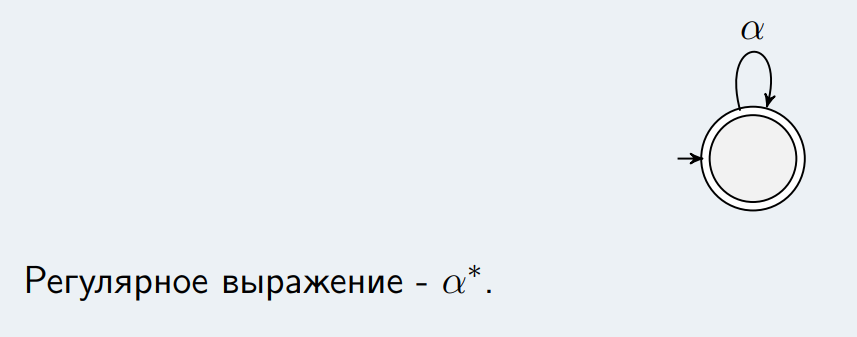
\includegraphics[scale=0.25]{assets/Q1RegexpAutomaton.png}
	      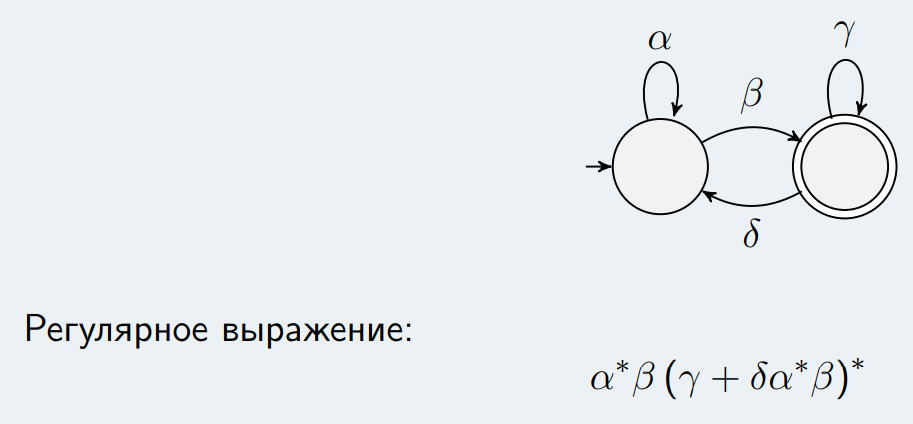
\includegraphics[scale=0.25]{assets/Q2RegexpAutomaton.png}
	\item Для перехода будем удалять нестартовые и незавешающие состояния:

	      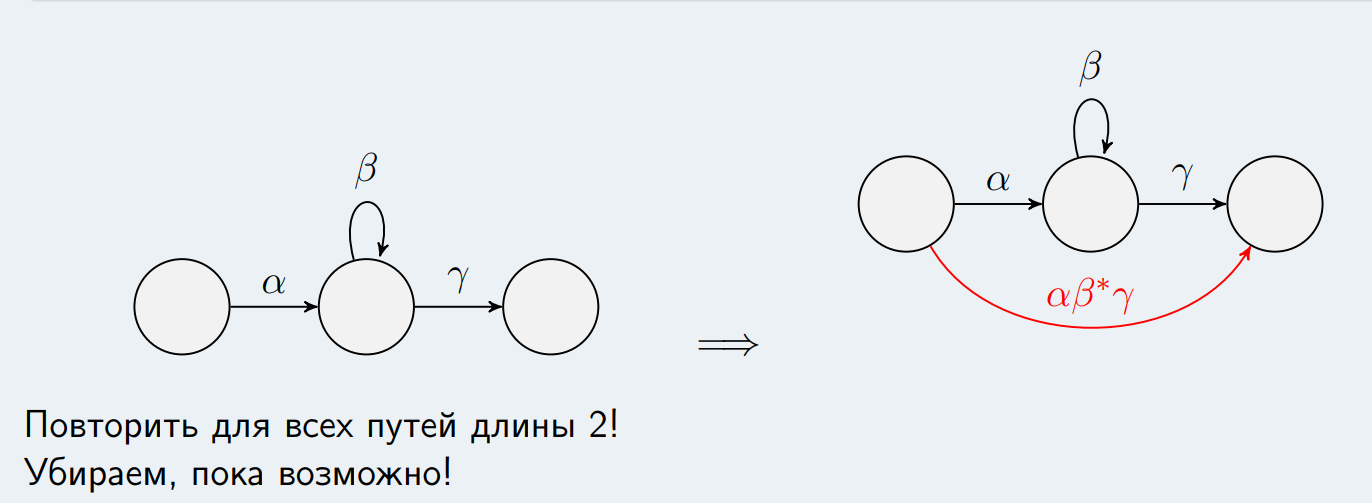
\includegraphics[scale=0.25]{assets/StepRegexpAutomaton.png}
\end{itemize}
\subsection{Про эквивалентные состояния ПДКА}
\subsubsection*{Эквивалентность состояний в ПДКА}
\begin{definition}
	Пусть $L \subset \Sigma^*$ -- автоматный язык, $M$ -- ПДКА для $L$. Тогда определим отношение $\sim_L$ на $\Sigma^*$:
	\[
		u \sim_L v \Leftrightarrow \forall w \in \Sigma^* :\: uw \in L \Leftrightarrow vw \in L
	\]
\end{definition}

\begin{proof}
	Проверим, что $\sim_L$ -- отношение эквивалентности:
	\begin{itemize}
		\item Рефлексивность: $uw \in L \Leftrightarrow uw \in L$
		\item Симметричность: $v \sim_L u:\: uw \in L \Leftrightarrow vw \in L$
		\item Транзитивность:
		      \begin{itemize}
			      \item $u \sim_L v :\: uw \in L \Leftrightarrow vw \in L$
			      \item $v \sim_L s :\: vw \in L \Leftrightarrow sw \in L$
			      \item $uw \in L \Leftrightarrow sw \in L \Rightarrow u \sim_L s$
		      \end{itemize}
	\end{itemize}
\end{proof}

\begin{definition}
	Определим $\sim_M$ над ПДКА:
	\[
		q_1 \sim_M q_2 \Leftrightarrow \forall w \in \Sigma^* :\: \Delta(q_1,\, w) \in F \Leftrightarrow \Delta(q_2,\, w) \in F
	\]
\end{definition}

\subsubsection*{Эквивалентность слов по языку}
\begin{definition}
	Мы можем разбить язык $\Sigma^*$ на классы эквивалентности по отношению $\sim_L$:
	\[
		\Sigma^* / \sim_L := \{\{u \:|\: u \sim_L v\} \:|\: v \in \Sigma^*\}
	\]
\end{definition}

\subsubsection*{Оценка на минимальное количество состояний в ПДКА.}
\begin{lemma}
	Пусть $L_q := \{w \:|\: \Delta(q_0,\, w) = q\}$. Тогда каждый класс эквивалентности в $\Sigma^* / \sim_L$ -- объединение классов в $L_q$.
\end{lemma}

\begin{proof}
	Пусть $u,\, v \in L_q \Rightarrow \Delta(q_0,\, u) = \Delta(q_0,\, v) = q$. Попробуем преобразовать множество достижимых вершин по произвольному слову $w$, используя это свойство:
	\[
		\Delta(q_0,\, uw) = \Delta(\Delta(q_0,\, u),\, w) = \Delta(q,\, w) = \Delta(q_0,\, vw)
	\]
	Рассмотрим цепочку эквивалентностей:
	\[
		uw \in L \Leftrightarrow \Delta(q_0,\, uw) \in F \Leftrightarrow \Delta(q_0,\, vw) \in F \Leftrightarrow vw \in L
	\]
	Что по определению даёт нам $u \sim_L v$.
\end{proof}

\begin{corollary}
	Получаем оценку снизу на количество вершин в автомате:
	\[
		\vert\Sigma^*/\sim_L\vert \leq \vert Q\vert
	\]
\end{corollary}

\subsection{Критерий минимальности количества состояний в ПДКА}
\begin{lemma}
	Для любого автоматного языка $L$ существует ПДКА $M'$, такой, что все состояния в $M'$ попарно неэквивалентны
\end{lemma}

\begin{proof}
	Построим автомат над классами $[q] \in Q / \sim_M$:
	\[M' = \langle Q/\sim_M,\, \Sigma,\, \Delta',\, [q_0],\, F'\rangle\]
	где:
	\begin{itemize}
		\item $\Delta' = \{\langle[q],\, a\rangle \to [\Delta(q,\,a)]\}$
		\item $F' = \{[q] \:|\: q \in F\}$
	\end{itemize}
	Необходимо доказать:
	\begin{itemize}
		\item Переходы согласованы
		\item Завершающие состояния согласованы
		\item Распознаваемые языки согласованы
		\item Состояния попарно неэквивалентны
	\end{itemize}
	Итак, приступим к доказательству каждого из пунктов:

	Переходы согласованы, т.е. $q_1 \in [q] \Rightarrow \Delta(q_1,\, a) \in [\Delta(q,\,a)]$:
	\begin{align*}
		q_1 \in [q] \Rightarrow \forall w:\: \Delta(q_1,\,w) \in F \Leftrightarrow \Delta(q,\,w) \in F \text{ в том числе: } \\
		\forall w = au:\: \Delta(q_1,\,au) \in F \Leftrightarrow \Delta(q,\, au) \in F \Rightarrow                           \\
		\forall u:\: \Delta(\Delta(q_1,\,a),\,u) \in F \Leftrightarrow \Delta(\Delta(q,\,a),\,u) \in F \Rightarrow           \\
		\Delta(q_1,\,a) \sim_M \Delta(q,\,a)
	\end{align*}
	Завершающие состояния согласованы, т.е. $q_1 \in [q],\, q \in F \Rightarrow q_1 \in F$:
	\begin{align*}
		q_1 \in [q] \Rightarrow \forall w:\: \Delta(q_1,\,w) \in F \Leftrightarrow \Delta(q,\,w) \in F \text{ в том числе: } \\
		(\Delta(q_1,\,\varepsilon) = q_1) \in F \Leftrightarrow (\Delta(q,\, \varepsilon) = q) \in F
	\end{align*}
	Совпадение языков, т.е. $\forall w :\: \Delta([q_0],\, w) = [\Delta(q_0,\,w)]$ индукцией по $|w|$:
	\begin{itemize}
		\item База уже доказана в предыдущих пунктах
		\item Пусть $w = ua$:
		      \begin{align*}
			      \Delta([q_0],\, ua) = \Delta(\Delta([q_0],\, u),\, a) = \Delta([\Delta(q_0,\, u)],\, a) = [\Delta(\Delta(q_0,\,u),\, a)] = [\Delta(q_0,\,ua)]
		      \end{align*}
	\end{itemize}
	Тогда:
	\begin{align*}
		w \in L(M) \Leftrightarrow \Delta(q_0,\, w) \in F \Leftrightarrow \Delta([q_0],\, w) \in F' \Leftrightarrow w \in L(M')
	\end{align*}
	Осталось показать, что все все состояния в получившемся автомате попарно неэквивалентны: пусть  $[q_1] \sim_{M'} [q_2]$, тогда
	\begin{align*}
		\forall w :\: \Delta([q_1],\, w) \in F' \Leftrightarrow \Delta([q_2],\,w) \in F' \Rightarrow \forall w :\: [\Delta(q_1,\,w)] \in F' \Leftrightarrow [\Delta(q_2,\,w)] \in F' \Rightarrow \\
		\forall w :\: \Delta(q_1,\, w) \in F \Leftrightarrow \Delta(q_2,\,w) \in F \Rightarrow                                                                                                   \\
		q_1 \sim_M q_2 \Rightarrow [q_1] = [q_2]
	\end{align*}

\end{proof}

\begin{theorem}
	$M$ -- минимальный ПДКА: $L(M) = L \Leftrightarrow$ Любые два состояния попарно неэквивалентны и все состояния достижимы из стартового
\end{theorem}

\begin{proof}
	($\Rightarrow$) Пусть $M$ -- минимальный ПДКА. Строим автомат $Q / \sim_M$: уменьшаем число состояний. Если в $M$ есть недостижимое состояние, то удаляем его.

	($\Leftarrow$) Из того, что в $M$ нет эквивалентных состояний:
	\begin{align*}
		\forall w_1,\, w_2 \in \Sigma^* :\: \Delta(q_0,\, w_1) \not\sim \Delta(q_0,\, w_2) \Rightarrow \exists u :\: \Delta(\Delta(q_0,\, w_1),\, u) \not\in F,\, \Delta(\Delta(q_0,\, w_2),\, u) \in F \Rightarrow \\
		\exists u :\: \Delta(q_0,\, w_1u) \not\in F,\, \Delta(q_0,\, w_2u) \in F \Rightarrow \exists u :\: w_1u \not\in L,\, w_2u \in L \Rightarrow                                                                 \\ w_1 \not\sim_L w_2
	\end{align*}
	Тогда $\vert\Sigma^*/\sim_L\vert \geq \vert Q\vert$, но $\forall$ ПДКА $M' :\: |\Sigma^*/\sim_L| \leq |Q'| \Rightarrow \vert Q\vert \leq \vert Q'\vert \Rightarrow M$ -- минимальный.
\end{proof}

\subsection{Про канонический ПДКА}
\begin{definition}
	$M_1$ и $M_2$ \textbf{изоморфны}, если существует биекция $\psi:\: Q_1 \to Q_2$:
	\begin{itemize}
		\item $\psi(q_0^1) = q_0^2$
		\item $\psi(F_1) = F_2$
		\item Если $\Delta(q_1,\, a) = q_2$, то $\Delta(\psi(q_1),\,a) = \psi(q_2)$
	\end{itemize}
\end{definition}

\subsubsection*{Канонический ПДКА - корректность построения}
Канонический ПДКА для языка $L$ определим, как $\Sigma^* / \sim_L$:
\begin{align*}
	M_0 = \langle\Sigma^*/\sim_L,\,\Sigma,\,\Delta,\, [\varepsilon],\,\{[w] \:|\: w \in L\} \rangle ;\;\;\;\; \Delta([u],\,a) = [ua],\, u \in \Sigma^*,\, a \in \Sigma
\end{align*}
Для корректности необходимо показать:
\begin{itemize}
	\item $u \sim_L v,\, u \in L \Rightarrow v \in L$
	\item $u \sim_L v \Rightarrow va \in [ua]$
\end{itemize}

\subsubsection*{Единственность минимального ПДКА}
\begin{lemma}
	Пусть $M$ -- минимальный ПДКА, тогда отображение $\psi$:
	\begin{itemize}
		\item $\psi:\: Q_M \to \Sigma^*/\sim_L$
		\item $\psi(q) = \{w \:|\: \Delta_M(q_0,\, w) = q\}$
	\end{itemize}
	является изоморфизмом.
\end{lemma}

\begin{proof}
	Необходимо доказать:
	\begin{itemize}
		\item $\psi(q_0) = [\varepsilon]$
		\item $\psi(F) = \{[w] \:|\: w \in L\}$
		\item Если $\Delta(q_1,\,a) = q_2$, то $\Delta(\psi(q_1),\, a) = \psi(q_2)$
	\end{itemize}

	Докажем биективность $\psi$: $\vert\Sigma^*/\sim_L\vert = \vert Q_M\vert \Rightarrow$ достаточно доказать инъективность:
	\begin{align*}
		\psi(q_1) = \psi(q_2) \Rightarrow \exists w :\: \Delta(q_0,\,w) = q_1,\, \Delta(q_0,\, w) = q_2 \Rightarrow q_1 = q_2
	\end{align*}
	Докажем согласованность стартовых состояний:
	\begin{align*}
		w \in \psi(q_0) \Rightarrow \Delta_M(q_0,\, w) = q_0 \text{ но мы знаем, что: } \\
		\Delta_M(q_0,\, \varepsilon) = q_0 \Rightarrow w \sim_L \varepsilon
	\end{align*}
	Согласованность завершающих состояний:
	\begin{align*}
		w \in \psi(q),\, q \in F \Rightarrow \Delta_M(q_0,\, w) = q \Rightarrow w \in L \Rightarrow [w] \in F'
	\end{align*}
	Осталось доказать согласованность переходов:
	\begin{align*}
		w \in \psi(q_1),\, \Delta(q_1,\,a) = q_2 \Rightarrow \Delta(q_0,\, w) = q_1 \Rightarrow \psi(q_1) = [w],\, \Delta([w],\, a) = [wa] \Rightarrow \\
		\Delta(q_0,\, wa) = \Delta(q_1,\,a) = q_2 \Rightarrow \psi(q_2) = [wa]
	\end{align*}
\end{proof}

\begin{theorem}
	МПДКА единственен с точностью до изоморфизма.
\end{theorem}

\begin{proof}
	Пусть $M_1,\, M_2$ -- ПДКА. Построим канонические изоморфизмы $\psi_1,\, \psi_2$. Тогда $\psi_2^{-1} \circ \psi_1$ -- изоморфизм $M_1$ в $M_2$.
\end{proof}

\subsection{Алгоритмы проверок}
\subsubsection*{Алгоритм проверки МПДКА на эквивалентность}
Необходимо получить неэквивалентные состояния, но у нас есть только слова. Как по ним понять, какие состояния попарно неэвивалентны? Ввести эквивалентность по словам малой длины.

\begin{definition}
	$q_1 \underset{n}{\sim} q_2$, если для любого слова $\vert w \vert \leq n$:
	\begin{align*}
		\Delta(q_1,\, w) \in F \Leftrightarrow \Delta(q_2,\, w) \in F
	\end{align*}
\end{definition}

\begin{lemma}
	\begin{align*}
		q_1 \sim q_2 \Leftrightarrow q_1 \underset{\vert Q \vert - 2}{\sim} q_2
	\end{align*}
\end{lemma}

\begin{proof}
	Покажем, если $\vert Q / \underset{i}{\sim}\vert = \vert Q / \underset{i + 1}{\sim}\vert$, то $\vert Q / \underset{i + 1}{\sim}\vert = \vert Q / \underset{i + 2}{\sim}\vert$.

	Очевидно, что $\vert Q / \underset{i + 1}{\sim}\vert \leq \vert Q / \underset{i + 2}{\sim}\vert$. По определению эквивалентности $q_1 \underset{i + 2}{\sim} q_2$:
	\begin{align*}
		\forall w = au,\, \vert w \vert \leq i + 2 :\: \Delta(q_1,\, au) \in F \Leftrightarrow \Delta(q_2,\,au) \in F \Rightarrow                                                          \\
		\forall a \in \Sigma :\: \Delta(q_1,\, a) \underset{i + 1}{\sim} \Delta(q_2,\, a) \overset{\vert Q / \underset{i}{\sim}\vert = \vert Q / \underset{i + 1}{\sim}\vert}{\Rightarrow} \\
		\forall a \in \Sigma :\: \Delta(q_1,\, a) \underset{i}{\sim} \Delta(q_2,\,a) \Rightarrow q_1 \underset{i + 1}{\sim} q_2
	\end{align*}
	Теперь понятно, что, если $\vert Q / \underset{i}{\sim}\vert = \vert Q / \underset{i + 1}{\sim}\vert$, то $\vert Q / \underset{i}{\sim}\vert = \vert Q / \sim \vert$

	Заметим, что $\vert Q / \sim_0\vert = \vert\{F,\, Q \setminus F\}\vert = 2$, но $\vert Q / \sim_i\vert$ неубывает и стабилизируется $\Rightarrow$
	\[
		\vert Q / \sim_i\vert \leq \vert Q / \sim\vert \leq \vert Q\vert
	\]
\end{proof}

\subsubsection*{Теорема Майхилла-Нероуда}
\begin{theorem}
	$L$ -- автоматный $\Leftrightarrow L$ содержит конечное количество классов эквивалентности $\Sigma^* / \sim_L$
\end{theorem}

\begin{proof}
	\begin{itemize}
		\item $\Rightarrow L$ -- автоматный, тогда $\vert\Sigma^* /\sim_L\vert \leq \vert Q \vert < +\infty$
		\item $\Leftarrow$ построим канонический МПДКА.
	\end{itemize}
\end{proof}

\subsection{Лемма о разрастании}
\subsubsection*{Лемма о разрастании для автоматных языков}
\begin{lemma}
	Пусть $L$ -- автоматный язык. Тогда
	\begin{align*}
		\exists P \: \forall w \in L :\: |w| \geq P \: \exists x,\,y,\,z:\: w = xyz,\, \vert xy \vert \leq P,\, |y| \neq 0 :\: \forall k \geq 0 :\: xy^kz \in L
	\end{align*}
\end{lemma}

\begin{proof}
	Построим $M$ -- НКА с 1-буквенными переходами: $L(M) = L$. Тогда $P := \vert Q \vert$. Если $\vert w \vert \geq P \Rightarrow$ посетили $\geq P + 1$ состояние.

	Значит $\exists q \in Q$, которую посетили дважды, значит мы можем ходить по этому циклу любое $k$ число раз.
\end{proof}

\subsubsection*{Пример неавтоматных языков}
\begin{example}
	\begin{align*}
		L = \{a^nb^n \:|\: n \in \mathbb{N}\}
	\end{align*}
\end{example}

\begin{proof}
	Неавтоматность доказывается отрицанием леммы о разрастании.
\end{proof}

\section{КС-грамматики и МП-автоматы}
\subsection{Про порождающие грамматики}
\subsubsection*{Порождающие грамматики}
\begin{definition}
	\textbf{Порождающая грамматика} $G = \langle N,\, \Sigma,\, P,\, S\rangle$, где:
	\begin{itemize}
		\item $N$ -- множество вспомогательных символов, $\vert N \vert < +\infty$
		\item $\Sigma$ -- алфавит -- множество терминальных символов, $\vert \Sigma \vert < +\infty,\, N \cap \Sigma = \emptyset$
		\item $S \in N$ -- стартовый нетерминал
		\item $P \subset ((N \cup \Sigma)^+ \setminus \Sigma^*) \times (N \cup \Sigma)^*$
	\end{itemize}
\end{definition}

\subsubsection*{Язык, задаваемый грамматикой}
\begin{definition}
	Отношением выводимости $\vdash_G$ называется наименьшее рефлексивное транзитивное отношение:
	\begin{align*}
		\forall (\alpha \to \beta) \in P,\, \forall \phi,\, \psi \in (N \cup \Sigma)^* :\: \phi\alpha\psi \vdash_G \phi\beta\psi
	\end{align*}
\end{definition}

\begin{definition}
	$w$ \textbf{выводимо в грамматике} $G = \langle N,\, \Sigma,\, P,\, S\rangle$, если $S \vdash_G w$
\end{definition}

\begin{definition}
	Языком $L$, порождённым грамматикой $G$ называется:
	\begin{align*}
		L(G) = L = \{w \:|\: S \vdash_G w\}
	\end{align*}
\end{definition}

\subsubsection*{Иерархия Хомского порождающих грамматик}
Разграничим грамматики по виду правил:
\begin{enumerate}
	\item Порождающие грамматики: любые правила
	\item Контекстно-зависимые грамматики: $\phi A \psi \to \phi\alpha\psi,\, \alpha \neq \varepsilon$
	\item Контекстно-свободные грамматики: $A \to \alpha$
	\item Праволинейные грамматики: $A \to wB,\, A \to w$
\end{enumerate}

При этом:
\begin{itemize}
	\item $A \in N,\, B \in N$ -- нетерминальные символы
	\item $\alpha,\, \phi,\, \psi \in (N \cup \Sigma)^*$
\end{itemize}

\subsection{Про праволинейные грамматики}
\subsubsection*{Праволинейные языки}
\begin{theorem}
	Множество автоматных языков равно множеству языков, задаваемых праволинейными грамматиками.
\end{theorem}

\begin{proof}
	Состояние в автомате -- нетерминалы в грамматике + сток
\end{proof}

\subsubsection*{Построение праволинейной грамматики по конечному автомату}
Пусть $M = \langle Q,\, \Sigma,\, \Delta,\, q_0,\, F\rangle$. Построим $G = \langle Q,\, \Sigma,\, P,\, q_0\rangle$, где:
\begin{align*}
	P = \{q_1 \to wq_2 \:|\: (\langle q_1,\, w\rangle \to q_2) \in \Delta\} \bigcup \{q \to \varepsilon \:|\: q \in F\}
\end{align*}

\begin{proof}
	Надо доказать два утверждения:
	\begin{enumerate}
		\item $\langle q_1,\, w\rangle \vdash_M \langle q_2,\, \varepsilon\rangle \Leftrightarrow q_1 \vdash_G wq_2$
		\item $\langle q_1,\, w\rangle \vdash_M \langle q,\, \varepsilon\rangle,\, q \in F \Leftrightarrow q_1 \vdash_G w$
	\end{enumerate}
	В начале докажем $\Rightarrow$ для обоих пунктов.

	Первый пункт доказывается индукцией по длине вывода в $M$.
	\begin{itemize}
		\item База индукции -- 0 шагов:
		      \begin{align*}
			      \langle q_1,\, w\rangle \vdash_M \langle q_2,\, \varepsilon\rangle \Rightarrow q_1 = q_2,\, w = \varepsilon \Rightarrow q_1 \vdash_G \varepsilon q_2
		      \end{align*}
		\item Для перехода представим произвольное слово $w = vu,\, u \in \Sigma$:
		      \begin{align*}
			      \langle q_1,\, w\rangle \vdash_M \langle q_3,\, v\rangle \vdash_{M,\, 1} \langle q_2,\, \varepsilon\rangle \Rightarrow q_1 \vdash_G uq_3,\, q_3 \vdash_G vq_2 \Rightarrow q_1 \vdash_G uvq_2 = wq_2
		      \end{align*}
	\end{itemize}
	Теперь второй пункт:
	\begin{align*}
		\langle q_1,\, w \rangle \vdash_M \langle q,\, \varepsilon\rangle,\, q \in F \Rightarrow q_1 \vdash_G wq,\, (q \to \varepsilon) \in P \Rightarrow q_1 \vdash_G w
	\end{align*}
	Теперь $\Leftarrow$ для обоих пунктов:

	Первый тоже докажем индукцией по длине вывода в $G$Ж
	\begin{itemize}
		\item База индукции 0 шагов:
		      \begin{align*}
			      q_1 \vdash_{G,\, 0} wq_2 \Rightarrow q_1 = q_2,\, w = \varepsilon \Rightarrow \langle q_1,\, \varepsilon\rangle \vdash_M \langle q_2,\, \varepsilon\rangle
		      \end{align*}
		\item Для перехода опять разложим $w = vu,\, u \in \Sigma$:
		      \begin{align*}
			      q_1 \vdash_G vq_3 \vdash_G wq_2 \Rightarrow \langle q_1,\, v\rangle \vdash_M \langle q_3,\, \varepsilon\rangle,\, \langle q_3,\, u\rangle \vdash_M \langle q_2,\, \varepsilon\rangle \Rightarrow \langle q_1,\, vu\rangle \vdash_M \langle q_3,\, u\rangle \vdash_{M,\, 1} \langle q_2,\, \varepsilon\rangle
		      \end{align*}
	\end{itemize}
	Второй пункт:
	\begin{align*}
		q_1 \vdash_G wq \vdash_{G,\, 1} w \Rightarrow \langle q_1,\, w\rangle \vdash_M \langle q,\, \varepsilon\rangle,\, q \vdash_{G,\, 1} \varepsilon \Rightarrow q \in F
	\end{align*}

	После доказательства двух пунктов нам становится очевидно, что следующие утверждения эквивалентны:
	\begin{itemize}
		\item $w \in L(M)$
		\item $\exists q \in F :\: \langle q_0,\, w\rangle \vdash \langle q,\, \varepsilon\rangle$
		\item $q_0 \vdash_G w$
		\item $w \in L_G$
	\end{itemize}
\end{proof}

\subsection{Построение конечного автомата по праволинейной грамматике}
Строим автомат:
\begin{align*}
	M = \langle N \cup \{q_f\},\, \Sigma,\, \Delta,\, S,\, \{q_f\}\rangle
\end{align*}
Переходы:
\begin{enumerate}
	\item $\langle A,\, w\rangle \to B$, если $(A \to wB) \in P$
	\item $\langle A,\, w\rangle \to q_f$, если $(A \to w) \in P$
\end{enumerate}

\begin{proof}
	Надо доказать два утверждения:
	\begin{enumerate}
		\item $\langle A,\, w\rangle \vdash_M \langle B,\, \varepsilon\rangle \Leftrightarrow A \vdash_G wB;\;\; A,\,B \in N$
		\item $\langle A,\, w\rangle \vdash_M \langle q_f,\, \varepsilon\rangle \Leftrightarrow A \vdash_G w$
	\end{enumerate}

	В начале докажем $\Rightarrow$ для обоих пунктов:

	Первый будем доказывать по индукции:
	\begin{itemize}
		\item База индукции -- 0 шагов:
		      \begin{align*}
			      \langle A,\, w\rangle \vdash_{M,\, 1} \langle B,\, \varepsilon\rangle \Rightarrow A = B,\, w = \varepsilon \Rightarrow A \vdash_G \varepsilon B
		      \end{align*}
		\item Для перехода представим произвольное слово $w = vu,\, u \in \Sigma$:
		      \begin{align*}
			      \langle A,\, w\rangle \vdash_M \langle C,\, u\rangle \vdash_{M,\,0} \langle B,\, \varepsilon\rangle \Rightarrow A \vdash_G vC,\, C \vdash_G uB \Rightarrow A \vdash_G vuB = wB
		      \end{align*}
	\end{itemize}
	Теперь второй пункт для произвольного $w = vu$:
	\begin{align*}
		\langle A,\, v\rangle \vdash_M \langle C,\, u\rangle \vdash_{M,\,1} \langle q_f,\, \varepsilon\rangle \Rightarrow A \vdash_G vC,\, C \vdash_G u \Rightarrow A \vdash_G vu = w
	\end{align*}
	Перейдём к доказательству $\Leftarrow$ для обоих пунктов:

	Первый пункт также будет доказан по индукции:
	\begin{itemize}
		\item База -- 0 шагов:
		      \begin{align*}
			      A \vdash_{G,\, 0} wB \Rightarrow w = \varepsilon,\, A = B \Rightarrow \langle A,\, \varepsilon\rangle \vdash_M \langle B,\, \varepsilon\rangle
		      \end{align*}
		\item Переход для произвольного $w = uv$:
		      \begin{align*}
			      A \vdash_G uC \vdash_{G,\,1} uvB \Rightarrow \langle A,\, u\rangle \vdash_M \langle C,\, \varepsilon\rangle,\, \langle C,\, v\rangle \vdash_M \langle B,\, \varepsilon\rangle \Rightarrow \langle A,\, uv\rangle \vdash_M \langle B,\, \varepsilon\rangle
		      \end{align*}
	\end{itemize}
	Второй пункт для $w = uv$:
	\begin{align*}
		A \vdash_G uC \vdash_{G,\,1} uv \Rightarrow \langle A,\, u\rangle \vdash_M \langle C,\, \varepsilon\rangle,\, \langle C,\, v\rangle \vdash \langle q_f,\, \varepsilon\rangle \Rightarrow \langle A,\, uv\rangle \vdash_M \langle q_f,\, \varepsilon\rangle
	\end{align*}

	После доказанных двух пунктов становится очевидным эквивалентность данных утверждений:
	\begin{itemize}
		\item $w \in L(M)$
		\item $\langle S,\, w\rangle \vdash_M \langle q_f,\, \varepsilon\rangle$
		\item $S \vdash_G w$
		\item $w \in L(G)$
	\end{itemize}
\end{proof}

\subsection{Про КС-грамматики}
\subsubsection*{Примеры контекстно-свободных языков}
\begin{example}
	\begin{align*}
		S \to aSb \\
		S \to \varepsilon
	\end{align*}
	Задаёт неавтоматный язык $\{a^nb^n \:|\: n \in \mathbb{N}\}$
\end{example}

\subsubsection*{Замкнутость КС-языков относительно простейших операций}
\begin{proposition}
	$L_1 \cup L_2$ является КС-языком
\end{proposition}

\begin{proof}
	Построим КС-грамматику для языка $L_1 \cup L_2$. Для этого рассмотрим соответствующие грамматики для $L_1,\, L_2$. Пусть стартовые символы в них имеют имена $S$ и $T$. Тогда стартовый символ для $L_1 \cup L_2$ обозначим за $S'$ и добавим правило $S' \to S \:|\: T$. Покажем, что $S' \vdash_G w \Leftrightarrow S \vdash_G w \lor T \vdash_G w$.

	$\Leftarrow$: Поскольку $S \vdash_G$ и есть правило $S' \vdash_G S$, то по транзитивности выводимости получаем, что $S' \vdash_G w$. Аналогично и для $T$.

	$\Rightarrow$: Пусть $S' \vdash_G w$. Поскольку $S' \vdash S \:|\: T$ -- единственные правила, в которых нетерминал $S'$ присутствует в левой части, то это означает, что либо $S' \vdash_G S \vdash_G w$, либо $S' \vdash_G T \vdash_G w$.
\end{proof}

\begin{proposition}
	$L_1L_2$ -- КС-язык
\end{proposition}

\begin{proof}
	Аналогично предыдущему случаю построим КС-грамматику для языка $L_1L_2$. Для этого добавим правило $S' \vdash_G ST$, где $S$ и $T$ -- стартовые символы языков $L_1$ и $L_2$ соответственно.
\end{proof}

\begin{proposition}
	$L^* = \bigcup_{i = 0}^\infty L^i$ -- КС-язык.
\end{proposition}

\begin{proof}
	Если $S$ -- стартовый символ КС-грамматики для языка $L$, то добавим в КС-грамматику для языка $L^*$ новый стартовый символ $S'$ и правила $S' \vdash_G SS' \:|\: \varepsilon$
\end{proof}

\subsection{Удаление непорождающих и недостижимых символов в алгоритме примедения к нормальной форме Хомского. Асимптотика приведённых шагов.}
\subsubsection*{Удаление непорождающих символов}
\begin{definition}
	Символ $Y \in N$ называется \textbf{порождающим}, если:
	\begin{align*}{
			\exists} w \in \Sigma^* :\: Y \vdash w
	\end{align*}
\end{definition}

Удаляем непорождающие символы $Z$ и все правила, содержащие символы $Z$ -- получаем $G_1$.

\begin{proposition}
	\begin{align*}
		L(G) = L(G_1)
	\end{align*}
\end{proposition}

\begin{proof}
	Включение $L(G_1) \subset L(G)$ очевидно, так как мы удалили нетерминалы, которые никак не влияли на вывод слов, поэтому язык не увеличился.

	Докажем $L(G) \subset L(G_1)$. Пусть $w \in L(G) \setminus L(G_1)$.

	Тогда существует непорождающий $Z$: $S \vdash \alpha Z \beta \vdash w$. Тогда если $w = w_1uw_2:\: \alpha \vdash w_1,\, Z \vdash u,\, \beta \vdash w_2 \Rightarrow Z$ -- порождающий, противоречие.
\end{proof}

\subsubsection*{Удаление недостижимых символов}
\begin{definition}
	Символ $D \in N$ называется \textbf{достижимым}, если существуют некоторые $\phi,\, \psi \in (N \cup \Sigma)^*$, такие, что:
	\begin{align*}
		S \vdash \phi D \psi
	\end{align*}
\end{definition}

Удаляем все недостижимые символы и все содержащие их правила -- получаем $G_2$.

\begin{proposition}
	\begin{align*}
		L(G_1) = L(G_2)
	\end{align*}
\end{proposition}

\begin{proof}
	Включение $L(G_2) \subset L(G_1)$ очевидно, так как удалили все нетерминалы, которые не участвовали в выводе, поэтому язык не увеличился.

	Теперь докажем $L(G_1) \subset L(G_2) \Rightarrow \exists w \in L(G_1) \setminus L(G_2) \Rightarrow$ существует недостижимый $U :\: S \vdash \alpha U \beta \vdash w \Rightarrow U$ -- достижимый. Противоречие.
\end{proof}

\begin{proposition}
	В $G_2$ не появилось непорождающих символов.
\end{proposition}

\begin{proof}
	Пусть $B$ стал новым непорождающим в $G_2$. Тогда:
	\begin{itemize}
		\item $B$ был достижимым в $G_1$.
		\item $B$ был порождающим в $G :\: B \vdash_G u$
	\end{itemize}
	На пути вывода $B \vdash u$ был недостижимый символ $C$. Но, тогда строим пусть $S \to B \to C$ -- противоречие!
\end{proof}

\subsubsection*{Асимптотика приведённых шагов (в терминах изначальной грамматики)}
\begin{enumerate}
	\item Для поиска непорождающих нетерминалов требуется запустить $\vert N \vert$ BFS-ов. Сложность $O(\vert N \vert (\vert N\vert + \vert E \vert))$
	\item Для поиска недостижимых нетерминалов требуется запустить один BFS из $S$. Сложность $O(\vert N\vert + \vert E \vert)$
\end{enumerate}

\subsection{Удаление длинных, смешанных правил и eps-порождающих символов. Асимптотика приведённых шагов.}
\subsubsection*{Удаление длинных правил}
Сделаем замену:
\[
	B \to A_1A_2\cdots A_n
\]
на:
\begin{align*}
	B \to A_1B_1   \\
	B_1 \to A_2B_2 \\
	\cdots         \\
	B_{n - 2} \to A_{n - 1}A_n
\end{align*}
Получим грамматику $G_3$.

\begin{note}
	Если в дереве вывода $G_3$ появился $B_k$, то в нём появятся все правила, в левых и правых частях которых есть $B_1,\,\cdots,\,B_{n-2}$.
\end{note}

\subsubsection*{Удаление смешанных правил}
Сделаем замену:
\[
	A \to A_1bA_2d
\]
на
\begin{align*}
	A \to A_1BA_2D \\
	B \to b        \\
	D \to d
\end{align*}
Получим грамматику $G_4$.

\subsubsection*{Удаление eps-порождающих}
\begin{definition}
	Символ $E$ называется $\varepsilon$-порождающим, если $E \vdash \varepsilon$.
\end{definition}

Сделаем замену:
\begin{itemize}
	\item Добавим правило $A \to B$, если $A \to BC,\, C \vdash \varepsilon$.
	\item Добавим правило $A \to C$, если $A \to BC,\, B \vdash \varepsilon$.
	\item Удалим правила $A \to \varepsilon$.
\end{itemize}
Получим грамматику $G_5$.

\begin{proposition}
	\begin{align*}
		L(G_4) = L(G_5)
	\end{align*}
\end{proposition}

\begin{proof}
	$L(G_4) \subset L(G_5)$ докажем индукцией по длине вывода:
	\begin{itemize}
		\item База -- 1 шаг: $w = a,\, (A \to a) \in P_{G_5}$
		\item Переход $A \vdash_{G_4,\,1}\alpha \vdash_{G_4} w$
		      \begin{itemize}
			      \item $\alpha = B \Rightarrow (A \to B) \in P_{G_5}$.
			      \item $\alpha = BC \Rightarrow B \vdash_{G_4} w_1,\, C \vdash_{G_4} w_2$.
			      \item Если $w_1 \neq \varepsilon,\, w_2 \neq \varepsilon$ -- применяем переход для $B,\, C$.
			      \item Если $w_1 = \varepsilon:\: A \vdash_{G_5,\,1} C \vdash_{G_5} w_2 = w$
		      \end{itemize}
	\end{itemize}
	$L(G_5) \subset L(G_4)$ также докажем индукцией по длине вывода:
	\begin{itemize}
		\item База -- 1 шаг: $w = a,\, (A \to a) \in P_{G_4}$
		\item Переход $A \vdash_{G_5,\,1} B \vdash_{G_5} w$:
		      \begin{itemize}
			      \item $(A \to B) \in P_{G_4} \Rightarrow A \vdash_{G_4,\,1} B \vdash_{G_4} w$
			      \item $(A \to BC) \in P_{G_4},\, C \vdash_{G_4} \varepsilon \Rightarrow A \vdash_{G_4,\,1} BC \vdash w\varepsilon = w$
		      \end{itemize}
	\end{itemize}


\end{proof}

\subsubsection*{Асимптотика приведённых шагов (в терминах изначальной грамматики)}
\begin{enumerate}
	\item Сложность удаления длинных правил $O(\vert P \vert \max_{p \in P}\vert p \vert)$.
	\item Сложность удаления смешанных правил можно оценить также.
	\item Сложность удаления $\varepsilon$-порождающих нетерминалов можно оценить, как $O(\vert P \vert h)$, где $h$ -- максимальная глубина вывода $\varepsilon$ для изначальной грамматики.
\end{enumerate}

\subsection{Обработка стартового состояния и удаление цепных правил. Асимптотика приведённых шагов.}
\subsubsection*{Обработка стартового состояния}
Мы доказали $L(G_5) = L(G_4) \setminus \{\varepsilon\}$:
\begin{itemize}
	\item Заводим новый нетерминал $S'$, делаем его стартовым
	\item Добавляем правило $S' \to S$
	\item Если $S \vdash \varepsilon$, то добавляем $S' \to \varepsilon$
\end{itemize}

Получили грамматику $L(G_6)$.

\subsubsection*{Удаление цепных правил}
Сделаем транзитивное замыкание:
\begin{align*}
	B \to B_1 \to B_2 \to \cdots \to B_n \to CD \:|\: a
\end{align*}
заменим на:
\begin{align*}
	B \to CD \:|\: a
\end{align*}
Дополнительно удалим правила вида $A \to B$.

Получили грамматику $L(G_7)$.

\begin{proposition}
	\begin{align*}
		L(G_6) = L(G_7)
	\end{align*}
\end{proposition}

\begin{proof}
	Полностью аналогично доказательству после удаления $\varepsilon$-порождающих.
\end{proof}

\subsubsection*{Асимптотики}
\begin{enumerate}
	\item Для обработки стартового состояния нужно понять, было ли оно $\varepsilon$-порождающим, то есть достаточно запустить BFS и проверить, дошли ли мы до правила, содержащего $\varepsilon$ в правой части -- $O(\vert N\vert + \vert P\vert)$
	\item Для удаления цепных правил требуется транзитивное замыкание, которое можно построить, используя алгоритм Флойда-Фалкерсона: $O(h^3)$, где $h$ -- максимальная глубина вывода.
\end{enumerate}

\subsection{Алгоритм Кока-Янгера-Касами синтаксического разбора для КС-грамматик}
Алгоритм построен на динамике по подотрезкам: заведём массив $d[A][i,\,j] = \mathbb{I}(A \vdash w[i : j])$, очевидно, что $w \in L(G) \Leftrightarrow d[S][0,\,\vert w \vert] = \text{True}$

Индукция по длине слова:
\begin{itemize}
	\item $A \vdash w[i : j]$. Тогда существуют $B,\, C:\: A \vdash_1 BC,\, B \vdash w[i : k],\, C \vdash w[k : j] \Rightarrow d[B][i : k] = \text{True},\, d[C][k : j] = \text{True}$
	\item $d[A][i:j] = \text{True}$. Тогда для некоторого midPosition сработал переключатель (см. код алгоритма). Делаем индукционный переход.
\end{itemize}

Асимптотика алгоритма -- $O(\vert N\vert^3\cdot \vert P\vert)$

\subsection{Лемма о разрастании для КС-языков}
\subsubsection*{Лемма о разрастании для КС-языков}
\begin{lemma}
	Пусть $L$ -- КС-язык. Тогда
	\begin{align*}
		\exists p :\: \forall w \in L :\: \vert w\vert \geq p :\: \exists x,\,u,\,y,\,v,\,z \in \Sigma^* :\: w = xuyvz :\: \\
		\vert uv\vert > 0,\, |uyv| \leq p :\: \forall k \geq 0 :\: xu^kyv^kz \in L
	\end{align*}
\end{lemma}

\begin{proof}
	Рассмотрим грамматику $G$ в нормальном форме Хомского: $L = L(G)$. Каждый уровень дерева вывода увеличивает длину слова не более, чем вдвое. Если $p = 2^{\vert N \vert}$, то $\vert w\vert \geq p \geq 2^{\vert N\vert}$. Тогда глубина дерева разбора более $\vert N\vert$ -- воспользуемся принципом Дирихле.

	Найдётся такой нетерминал $A$:
	\begin{align*}
		S \vdash xAz \vdash xuAvz \vdash xuyvz ;\;\;\;\;\; A \vdash uAv
	\end{align*}
	Среди таких $A$ рассмотрим такое, что его глубина относительно корня наибольшая. Тогда $|uyv| \leq 2^{\vert N\vert} = p$ (иначе были бы повторения)
\end{proof}

\subsubsection*{Пример не КС-языка}
\begin{example}
	Язык
	\begin{align*}
		\{a^nb^nc^n \:|\: n \in \mathbb{Z}^+\}
	\end{align*}
	не является КС-языком.
\end{example}

\begin{proof}
	Воспользуемся отрицанием леммы о разрастании.
\end{proof}

\subsection{МП-автомат}
\begin{definition}
	\textbf{Автомат с магазинной памятью} -- МП-автомат:
	\begin{itemize}
		\item $Q$ -- множество состояний, $\vert Q\vert < +\infty$
		\item $\Sigma$ -- алфавит, $\vert \Sigma\vert < +\infty$
		\item $\Gamma$ -- стековый алфавит, $\vert \Gamma\vert < +\infty,\, \Gamma \cap \Sigma = \emptyset$
		\item $\Delta \subset (Q \times \Sigma^* \times \Gamma^*) \times (Q \times \Gamma^*),\, \vert \Delta\vert < +\infty$
		\item $q_0 \in Q$ -- стартовое состояние.
		\item $F \subset Q$ -- множество завершающих состояний.
	\end{itemize}
\end{definition}

\begin{definition}
	\textbf{Конфигурацией в МП-автомате} называется тройка $\langle q,\, u,\, \gamma\rangle \in Q \times \Sigma^* \times \Gamma^*$.
\end{definition}

\begin{definition}
	$\vdash$ -- наименьшее рефлексивное транзитивное отношение, что
	\[
		\forall\langle q_1,\,u,\,\theta\rangle \to \langle q_2,\, \beta\rangle \in \Delta :\: \forall v \in \Sigma^*,\, \eta \in \Gamma^* \: \langle q_1,\, uv,\, \eta\alpha\rangle \vdash \langle q_2,\, v,\, \eta\beta\rangle
	\]
\end{definition}

\begin{definition}
	Языком, распознаваемым МП-автоматом, называется
	\[
		L(M) = \{w \in \Sigma^* \:\vert\: \exists q \in F :\: \langle q_0,\, w,\, \varepsilon\rangle \vdash \langle q,\, \varepsilon,\, \varepsilon\rangle\}
	\]
\end{definition}

\begin{proposition}
	Для любого МП-автомата существует эквивалентный МП-автомат, для которого выполнено соотношение:
	\[
		\forall \langle q_1,\, u,\, \alpha\rangle \to \langle q_2,\, \beta\rangle \in \Delta :\: \vert u\vert \leq 1,\, \vert\alpha\vert + \vert\beta\vert \leq 1
	\]
\end{proposition}

\begin{proof}
	Действие "считать $n$ букв со входа" растягиваем в "считать $n$ раз 1 букву со входа".

	Действие "снять со стека $n$ букв и положить на него $m$ букв" растягиваем в "снять $n$ раз со стека $1$ букву, положить $m$ раз на стек $1$ букву".
\end{proof}

\begin{proposition}
	Для любого МП-автомата существует эквивалентный МП-автомат, для которого выполнено соотношение:
	\[
		\forall \langle q_1,\, u,\, \alpha\rangle \to \langle q_2,\, \beta\rangle \in \Delta :\: \vert u\vert \leq 1,\, \vert\alpha\vert + \vert\beta\vert = 1
	\]
\end{proposition}

\begin{proof}
	Аналогично предыдущему утверждению, однако останутся переходы
	\[
		\langle q_1,\, w,\, \varepsilon\rangle \to \langle q_2,\, \varepsilon\rangle \in \Delta
	\]
	Вводим dummy стековый элемент $T$ и превращаем переход выше в два последовательных перехода
	\[
		\langle q_1,\, w,\, \varepsilon\rangle \to \langle q',\,T\rangle,\, \langle q',\,\varepsilon,\, T\rangle \to \langle q_2,\, \varepsilon\rangle
	\]
\end{proof}

\subsection{Построение МП-автомата по КС-грамматике}
\begin{theorem}
	Для любой КС-грамматики $G$ существует МП-автомат $M$:
	\[
		L(M) = L(G)
	\]
\end{theorem}

\begin{proof}
	Пусть $G = \langle N,\, \Sigma,\, P,\, S\rangle$, определим автомат
	\[
		M = \langle \{q_0,\, q_1\},\, \Sigma,\, N \cup \Sigma,\, \Delta,\, q_0,\, \{q_1\}\rangle
	\]
	причём $\Delta$ состоит из правил:
	\begin{itemize}
		\item $\langle q_0,\, \varepsilon,\, S\rangle \to \langle q_1,\, \varepsilon\rangle$
		\item $\langle q_0,\, \varepsilon,\, \alpha\rangle \to\langle q_0,\, A\rangle$, если $A \to \alpha \in P$
		\item $\langle q_0,\, a,\, \varepsilon\rangle \to \langle q_1,\, a\rangle,\, a \in \Sigma$
	\end{itemize}
	Хотим доказать, что
	\[
		\alpha \vdash w \Leftrightarrow \langle q_0,\, w,\, \varepsilon\rangle \vdash_M \langle q_0,\, \varepsilon,\, \alpha\rangle
	\]
	Вначале для $\Rightarrow$:

	Индукция по длине вывода:
	\begin{itemize}
		\item База $\alpha \vdash_0 w$. Тогда $\alpha = a = w \Rightarrow \langle q_0,\, a,\, \varepsilon\rangle \vdash \langle q_0,\, \varepsilon,\, a\rangle$ по третьему типу правил.
		\item Для перехода рассмотрим $A \vdash_1 \alpha_1\cdots\alpha_k \vdash w_1\cdots w_k = w$, где $\alpha_i$ -- нетерминалы, а $w_i$ -- ерминалы
		\item По предположению, $\langle q_0,\, w_j,\, \varepsilon\rangle \vdash \langle q_0,\, \varepsilon,\, \alpha_j\rangle$
		\item Тогда
		      \[
			      \langle q_0,\, w_1\cdots w_k,\, \varepsilon\rangle \vdash \langle q_0,\, w_2\cdots w_k,\, \alpha_1\rangle\vdash\cdots\vdash\langle q_0,\, \varepsilon,\, \alpha_1\cdots\alpha_k\rangle \vdash\langle q_0,\, \varepsilon,\, A\rangle
		      \]
	\end{itemize}
	Теперь $\Leftarrow$:

	Индукция по длине вывода:
	\begin{itemize}
		\item База: 1 шаг
		      \begin{itemize}
			      \item $\langle q_0,\, a,\, \varepsilon\rangle \vdash \langle q_0,\, \varepsilon,\, a\rangle \Rightarrow a \vdash a$
			      \item $\langle q_0,\, \varepsilon,\, \varepsilon\rangle\vdash\langle q_0,\, \varepsilon,\, A\rangle \Rightarrow A \to \varepsilon \in P$
		      \end{itemize}
		\item Переход: $\langle q_0,\, w,\, \varepsilon\rangle\vdash\langle q_0,\, \varepsilon,\, \alpha_1\cdots\alpha_k\rangle\vdash_1\langle q_0,\, \varepsilon,\, A\rangle$
		      \begin{itemize}
			      \item При этом $A \to \alpha_1\cdots\alpha_k \in P$
			      \item Найдём момент, когда на стеке появится $\alpha_1$: $\langle q_0,\, w,\, \varepsilon\rangle \vdash\langle q_0,\, w',\, \alpha_1\rangle$
			      \item Тогда $w = u_1w'$, причём $\langle q_0,\, u_1,\, \varepsilon\rangle \vdash\langle q_0,\, \varepsilon,\, \alpha_1\rangle$. Тогда $\alpha_1 \vdash u_1$.
			      \item Аналогично, $\alpha_j \vdash u_j$ и $A \vdash \alpha_1\cdots\alpha_k \vdash w$
		      \end{itemize}
	\end{itemize}
	Для доказательства совпадения языков остаётся заметить эквивалентность следующих фактов:
	\begin{itemize}
		\item $w \in L(M)$
		\item $\langle q_0,\,w,\, \varepsilon\rangle\vdash\langle q_1,\, \varepsilon,\, \varepsilon\rangle$
		\item $\langle q_0,\, w,\, \varepsilon\rangle \vdash \langle q_0,\, \varepsilon,\, S\rangle \vdash\langle q_1,\, \varepsilon,\, \varepsilon\rangle$
		\item $S \vdash w$
		\item $w \in L(G)$
	\end{itemize}
\end{proof}

\subsection{Построение КС-грамматики по МП-автомату}
\begin{theorem}
	Каждому МП-автомату $M$ соответствует КС-грамматика $G$:
	\[
		L(M) = L(G)
	\]
\end{theorem}

\begin{proof}
	Определим множество нетерминалов $N$, как
	\[
		N = \{A_{ij} \:\vert\: q_i,\, q_j \in Q\} \cup S
	\]
	Правила будем строить так:
	\begin{itemize}
		\item $A_{ij} \to uA_{st}vA_{rj}$, если
		      \begin{itemize}
			      \item $\langle q_i,\, u,\, \varepsilon\rangle\to\langle q_s,\, A\rangle$
			      \item $\langle q_t,\,v,\,A\rangle\to\langle q_r,\, \varepsilon\rangle$
		      \end{itemize}
		\item $A_{ij} \to \varepsilon$
		\item $S \to A_{0j}$, если $q_j \in F$
	\end{itemize}
	Хотим показать, что
	\[
		A_{ij} \vdash w \Leftrightarrow \langle q_i,\, w,\, \varepsilon\rangle \vdash\langle q_j,\, \varepsilon,\, \varepsilon\rangle
	\]
	В начале $\Rightarrow$:
	\begin{itemize}
		\item База: $A_{ij} \vdash_1 w$. Тогда $w = \varepsilon,\, i = j$. Значит, $\langle q_i,\, w,\, \varepsilon\rangle \vdash \langle q_j,\, \varepsilon,\,\varepsilon\rangle$
		\item Переход: $A_{ij} \vdash_1 uA_{st}vA_{rj} \vdash uzvy$
		      \begin{itemize}
			      \item По построению 			$\langle q_i,\, u,\, \varepsilon\rangle\to\langle q_s,\, A\rangle$, $\langle q_t,\,v,\,A\rangle\to\langle q_r,\, \varepsilon\rangle$
			      \item По предположению: $A_{st} \vdash z \Rightarrow \langle q_s,\, z,\, \varepsilon\rangle \vdash\langle q_t,\, \varepsilon,\, \varepsilon\rangle$ и $A_{rj} \vdash y \Rightarrow \langle q_r,\, y,\, \varepsilon\rangle\vdash\langle q_j,\, \varepsilon,\, \varepsilon\rangle$
			      \item Тогда в итоге
			            \[
				            \langle q_i,\, w,\, \varepsilon\rangle \vdash \langle q_i,\, uzvy,\, \varepsilon\rangle \vdash \langle q_s,\, zvy,\, A\rangle \vdash \langle q_t,\, vy,\, A\rangle \vdash \langle q_r,\, y,\, \varepsilon\rangle \vdash \langle q_j,\, \varepsilon,\, \varepsilon\rangle
			            \]
		      \end{itemize}
	\end{itemize}
	Теперь для $\Leftarrow$:
	\begin{itemize}
		\item База: $\langle q_i,\, w,\, \varepsilon\rangle \vdash_0\langle q_j,\, \varepsilon,\, \varepsilon\rangle$. Тогда $i = j,\, w =\varepsilon,\, A_{ii} \to \varepsilon$
		\item Переход: $\langle q_i,\, w,\, \varepsilon\rangle\vdash\langle q_j,\, \varepsilon,\, \varepsilon\rangle$
		      \begin{itemize}
			      \item Идя по цепочке вывода, $\exists w = uzvy$, причём
			            \[
				            \langle q_i,\, w,\, \varepsilon\rangle \vdash \langle q_i,\, uzvy,\, \varepsilon\rangle \vdash \langle q_s,\, zvy,\, A\rangle \vdash \langle q_t,\, vy,\, A\rangle \vdash \langle q_r,\, y,\, \varepsilon\rangle \vdash \langle q_j,\, \varepsilon,\, \varepsilon\rangle
			            \]
			      \item По предположению: $A_{st} \vdash z \Leftarrow \langle q_s,\, z,\, \varepsilon\rangle \vdash\langle q_t,\, \varepsilon,\, \varepsilon\rangle$ и $A_{rj} \vdash y \Leftarrow \langle q_r,\, y,\, \varepsilon\rangle\vdash\langle q_j,\, \varepsilon,\, \varepsilon\rangle$
			      \item Тогда
			            \[
				            A_{ij} \vdash uA_{st}vA_{rj} \vdash uzvy = w
			            \]
		      \end{itemize}
	\end{itemize}
	Для доказательства теоремы заметим эквивалентность следующих утверждений:
	\begin{itemize}
		\item $w \in L(G)$
		\item $S \vdash w$
		\item $\exists q_j \in F :\: S \vdash A_{0j} \vdash w$
		\item $\exists q_j \in F :\: \langle q_0,\,w,\,\varepsilon\rangle\vdash\langle q_j,\,\varepsilon,\,\varepsilon\rangle$
		\item $w \in L(M)$
	\end{itemize}
\end{proof}

\subsection{Нормальная форма ГРейбах для КС-грамматик}
\begin{definition}
	КС-грамматика находится в нормальной форме Грейбах, если все правила имеют такой и только такой вид:
	\begin{itemize}
		\item $A \to a,\, a \in \Sigma$
		\item $A \to aB,\, A \in \Sigma;\, B \in N;\, B \neq S$
		\item $A \to aBC,\, A \in \Sigma;\, B,\, C \in N;\, B,\, C \neq S$
		\item $S \to \varepsilon$
	\end{itemize}
\end{definition}

\begin{theorem}
	Любая КС-грамматика может быть представима в НФ Грейбах
\end{theorem}

\begin{proof}
	Определим оператор левого деления
	\[
		B \setminus A := \{w \in \Sigma^* \:\vert\: \exists x \in B :\: xw \in A\}
	\]
	По исходной грамматике $G = \langle N,\, \Sigma,\, P,\, S\rangle$ построим
	\[
		G_g = \langle\{S\} \cup \{B \setminus A \:\vert\: A,\, B \in N\},\, \Sigma,\, P_g,\, S\rangle
	\]
	Как будут выглядеть правила новой грамматики?
	\begin{itemize}
		\item $S \to a(A \setminus S)$, если $A \to a$
		\item $A \setminus A \to \varepsilon,\, A \in N$
		\item $B \setminus A \to e(E \setminus D)(C \setminus A)$, если $C \to BD$ и $E \to e$
	\end{itemize}
	По сути, должны доказать
	\[
		B \setminus A \vdash w \Leftrightarrow A \vdash Bw
	\]
	В начале $\Rightarrow$:

	Индукция по длине вывода
	\begin{itemize}
		\item База: $B \setminus A \vdash_1 w$. Тогда $A = B,\, w = \varepsilon$. Значит, $A \vdash A\varepsilon$.
		\item Переход: $B \setminus A \vdash_1 e(E \setminus D)(C \setminus A) \vdash euv$.
		      \begin{itemize}
			      \item По предположению: $E \setminus D \vdash u \Rightarrow D \vdash Eu$, $C \setminus A \vdash v \Rightarrow A \vdash Cv$
			      \item По условию $C \vdash BD$
			      \item $A \vdash Cv \vdash BDv \vdash BEuv \vdash Beuv \vdash Bw$
		      \end{itemize}
	\end{itemize}
	Теперь $\Leftarrow$:

	Индукция по длине вывода:
	\begin{itemize}
		\item База: $A \vdash_0 Bw$. Тогда $A = B,\, w = \varepsilon$. Значит, $A \setminus A \vdash \varepsilon$.
		\item Переход: смотри картинку

		      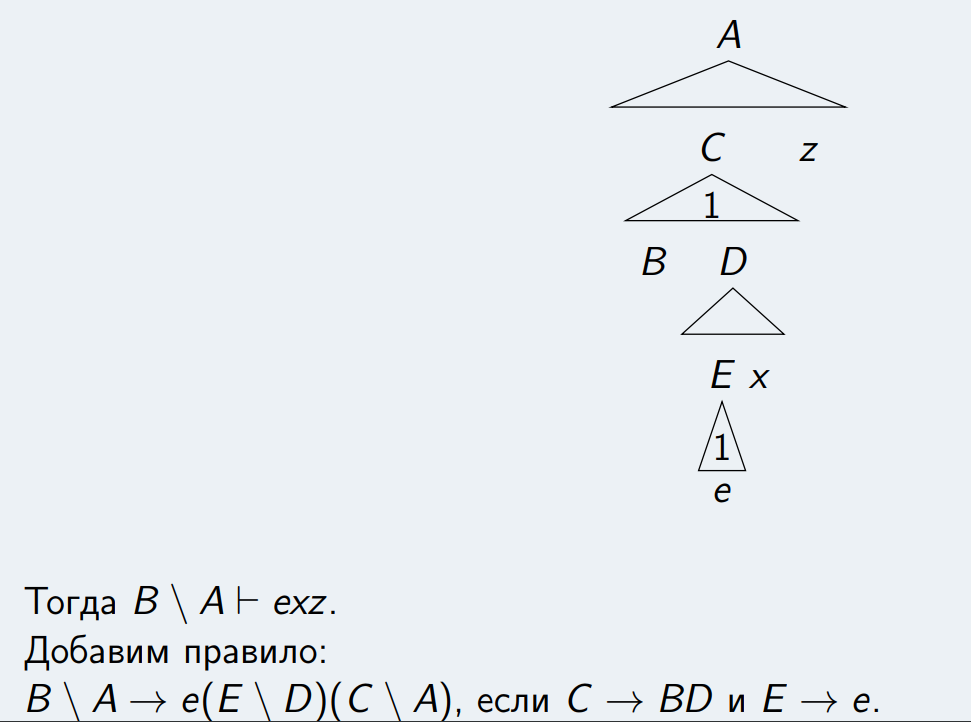
\includegraphics[scale=0.3]{assets/greibach.png}
	\end{itemize}

	Осталось доказать равенство языков, для этого приведём изначальную грамматику к нормальной форме Хомского $G_h$.

	Если $\varepsilon \in L(G_h)$, то $\varepsilon \in L(G_g)$ по правилу $S \to \varepsilon$.

	Пусть $w = au,\, a \in \Sigma$. Следующие утверждения эквивалентны:
	\begin{itemize}
		\item $au \in L(G_h)$
		\item $\exists A \to a :\: S \vdash Au \vdash_1 au$
		\item $\exists A \to a :\: S \vdash a(A \setminus S) \vdash au$
		\item $au \in L(G_g)$
	\end{itemize}
	Осталось убрать правила $A \setminus A \to \varepsilon$: аналогично удалению $\varepsilon$-порождающих.
\end{proof}

\begin{note}
	Аналогично можем определить обратную нормальную форму Грейбах с правилами вида:
	\begin{itemize}
		\item $A \to a$
		\item $A \to Ba$
		\item $A \to CBa$
		\item $S \to \varepsilon$
	\end{itemize}
\end{note}

\subsection{Построение МП-автомата без eps-переходов}
\begin{theorem}
	Для любого МП-автомата существует эквивалентный МП-автомат, для которого выполнено соотношение:
	\[
		\forall (\langle q_1,\, u,\, \alpha\rangle\to\langle q_2,\, \beta\rangle) \in \Delta :\: \vert u\vert = 1
	\]
\end{theorem}

\begin{proof}
	Рассмотрим алгоритм "КС-грамматика $\to$ МП-автомат" для обратной нормальной формы Грейбах!

	Хотим доказать, что
	\[
		\langle q_0,\, w,\, \varepsilon\rangle\vdash\langle q_0,\, \varepsilon,\, A\rangle \Leftrightarrow A \vdash w \: (A \neq S)
	\]
	Вначале $\Leftarrow$:
	\begin{itemize}
		\item $w \in L(G)$
		\item $S \vdash \varepsilon \Leftrightarrow \langle q_0,\, \varepsilon,\, \varepsilon\rangle \vdash\langle q,\, \varepsilon,\, \varepsilon\rangle \: (q \in F)$
		\item $S \vdash_1 CBA \vdash vua$:
		      \begin{itemize}
			      \item $C \vdash v \Rightarrow \langle q_0,\, vua,\, \varepsilon\rangle \vdash \langle q_0,\, ua,\, C\rangle$
			      \item $B \vdash u \Rightarrow \langle q_0,\, ua,\, C\rangle \vdash \langle q_0,\, a,\, CB\rangle$
			      \item $\langle q_0,\, a,\, CB\rangle \vdash_1\langle q_1,\, \varepsilon,\, \varepsilon\rangle$
		      \end{itemize}
	\end{itemize}
	Теперь $\Rightarrow$:
	\begin{itemize}
		\item $w \in L(G)$
		\item $S \vdash \varepsilon \Leftrightarrow \langle q_0,\, \varepsilon,\, \varepsilon\rangle \vdash\langle q,\, \varepsilon,\, \varepsilon\rangle \: (q \in F)$
		\item $\langle q_0,\, w,\, \varepsilon\rangle\vdash\langle q_1,\, \varepsilon,\, \varepsilon\rangle$:
		      \begin{itemize}
			      \item $w = xa,\, \langle q_0,\, a,\, CB\rangle \vdash_1\langle q_1,\, \varepsilon,\, \varepsilon\rangle$
			      \item Тогда $\exists x = vu :\: \langle q_0,\, ua,\, C\rangle \vdash\langle q_0,\, a,\, CB\rangle;\; \langle q_0,\, vua,\, \varepsilon\rangle \vdash \langle q_0,\, ua,\, C\rangle$
			      \item Значит $B \vdash u,\, C \vdash v$
			      \item $S \vdash CBa \vdash vua = w$
		      \end{itemize}
	\end{itemize}
\end{proof}

\subsection{КС-языки и теоретико-множественные операции}
\begin{proposition}
	КС-языки замкнуты относительно пересечения с регулярными языками
\end{proposition}

\begin{proof}
	Пусть $M = \langle Q,\, \Sigma,\, \Delta_M,\, q_0,\, D_M\rangle,\, L(M) = R$ -- НКА с 1-буквенными переходами.

	$MP = \langle P,\, \Sigma,\, \Gamma,\, \Delta_P,\, p_0,\, F_P\rangle,\, L(MP) = L$ -- МП-автомат с 1-буквенными переходами.

	Построим МП-автомат как декартово произведение НКА со стеком:
	\[
		M_i = \langle Q \times P,\, \Sigma,\, \Gamma,\, \Delta,\, (q_0,\, p_0),\, F_M \times F_p\rangle
	\]
	где $\Delta$ состоит из $\langle(q_1,\, p_1),\, a,\,\alpha\rangle \to\langle (q_2,\, p_2),\, \beta\rangle$, если:
	\begin{itemize}
		\item $\langle q_1,\, a\rangle \to q_2 \in \Delta_M$
		\item $\langle p_1,\,a,\,\alpha\rangle\to\langle p_2,\, \beta\rangle \in \Delta_P$
	\end{itemize}
\end{proof}

\section{Парсеры}
\subsection{Корректность алгоритма Эрли}
\begin{definition}
	Для каждого правила $A \to \alpha\beta$ определим ситуацию:
	\begin{align*}
		(A \to \alpha\cdot\beta,\, i) \in D_j,\, i \in [0 : \vert w\vert],\, j \in [0 : \vert w\vert]
	\end{align*}
	где $i$ отвечает за то, сколько букв было прочитано до "захода" в это правила, а $j$ за то, сколько букв прочитано на момент символа $\cdot$.
\end{definition}

На протяжении всего алгоритма используем 3 операции:
\begin{itemize}
	\item Scan -- читаем букву
	\item Predict -- спускаемся вниз
	\item Complete -- поднимаемся вверх
\end{itemize}

Добавим правило $S' \to S$, тогда стартовой ситуацией определим
\begin{align*}
	(S' \to \cdot S,\, 0) \in D_0
\end{align*}
а финальной будет
\begin{align*}
	(S' \to S\cdot,\, 0) \in D_{\vert w\vert}
\end{align*}

Корректность вывода при наличии ситуации гарантируется леммой:
\begin{lemma}
	Каждой ситуации соответствует вывод:
	\begin{align*}
		(A \to \alpha\cdot\beta,\, i) \in D_j \Leftrightarrow \exists \psi \in (N \cup \Sigma)^* :\: \alpha \vdash w[i : j] \\
		S' \vdash w[0:i]A\psi \vdash_1 w[0:i]\alpha\beta\psi
	\end{align*}
\end{lemma}

\begin{proof}
	Докажем индукцией по количеству эффективных шагов в алгоритме:
	\begin{itemize}
		\item База
		      \begin{itemize}
			      \item Появилась ситуация $(S' \to \cdot S,\, 0) \in D_0$
			      \item $S' \vdash \varepsilon w[0 : 0]S' \varepsilon = w[0:0]S\varepsilon,\, \alpha = \varepsilon = w[0 : 0]$
		      \end{itemize}
		\item Переход при Scan
		      \begin{itemize}
			      \item $(A \to \alpha\cdot a \beta,\, i) \in D_j,\, w[j] = a \Rightarrow (A \to \alpha a \cdot \beta,\, i) \in D_{j + 1}$
			      \item Предположение: $S' \vdash w[0:i]A\psi \vdash_1 w[0:i]\alpha a \beta\psi$
			      \item $\alpha \vdash w[i : j],\, \alpha a \vdash w[i : j + 1]$
		      \end{itemize}
		\item Переход при Predict
		      \begin{itemize}
			      \item $(B \to \cdot\gamma,\, j) \in D_j$ появилась при Predict после ситуации $(A \to \alpha\cdot B \beta,\, i) \in D_j$
			      \item Предположение $S' \vdash w[0:i]A\psi \vdash_1 w[0:i]\alpha B \beta\psi$
			      \item $\alpha \vdash w[i:j] \Rightarrow w[0:i]\alpha \vdash w[0:j]$
			      \item $S' \vdash w[0:i]\alpha B\beta\psi \vdash w[0:j]B\beta\psi \vdash_1 w[0:j]\gamma\beta\psi$
		      \end{itemize}
		\item Переход при Complete
		      \begin{itemize}
			      \item $(A \to \alpha B \cdot\beta,\, i) \in D_j$ появилась после ситуаций: $\exists k :\: (A \to \alpha\cdot B \beta,\, i) \in D_k;\;\; \exists (B \to \gamma\cdot,\, k) \in D_j$
			      \item Предположение $S' \vdash w[0:i]A\psi \vdash_1 w[0:i]\alpha B\beta\psi,\, \alpha \vdash w[i:k]$
			      \item Предположение 2: $B \vdash_1 \gamma \vdash w[k:j]$
			      \item Итого $\alpha B \vdash w[i:k]w[k:j] = w[i:j]$
		      \end{itemize}
	\end{itemize}
\end{proof}

\subsection{Полнота алгоритма Эрли}
Каждому выводу соответствует ситуация:

\begin{align*}
	S' \vdash_k w[0:i]A\psi \vdash_1 w[0:i]\alpha\beta\psi,\, \alpha\vdash_l w[i:j]
\end{align*}
идукцией по $(j,\, l + k,\, l)$
\begin{itemize}
	\item База $j = 0,\, k + l = 0$
	      \begin{itemize}
		      \item $l = 0 \Rightarrow \alpha = \varepsilon$
		      \item $k = 0 \Rightarrow w[0:i] = \varepsilon,\, A = S'$
		      \item $S' \to S \Rightarrow (S' \to \cdot S,\, 0) \in D_0$
	      \end{itemize}
	\item Переход: рассмотрим последний символ $\alpha$. Возможны 3 случая:
	      \begin{enumerate}
		      \item $\alpha = \alpha' b$:
		            \begin{itemize}
			            \item $\alpha' \vdash_l w[i : j-1],\, w[j] = b$
			            \item $S' \vdash w[0:i]\alpha'b\beta\psi$
			            \item Предположение $(j - 1,\, k+l,\,k):\: (A \to \alpha'\cdot bB,\, i) \in D_{j - 1}$
			            \item $(A \to \alpha'b\cdot B,\, i) \in D_j$ по Scan
		            \end{itemize}
		      \item $\alpha = \alpha' B$

		            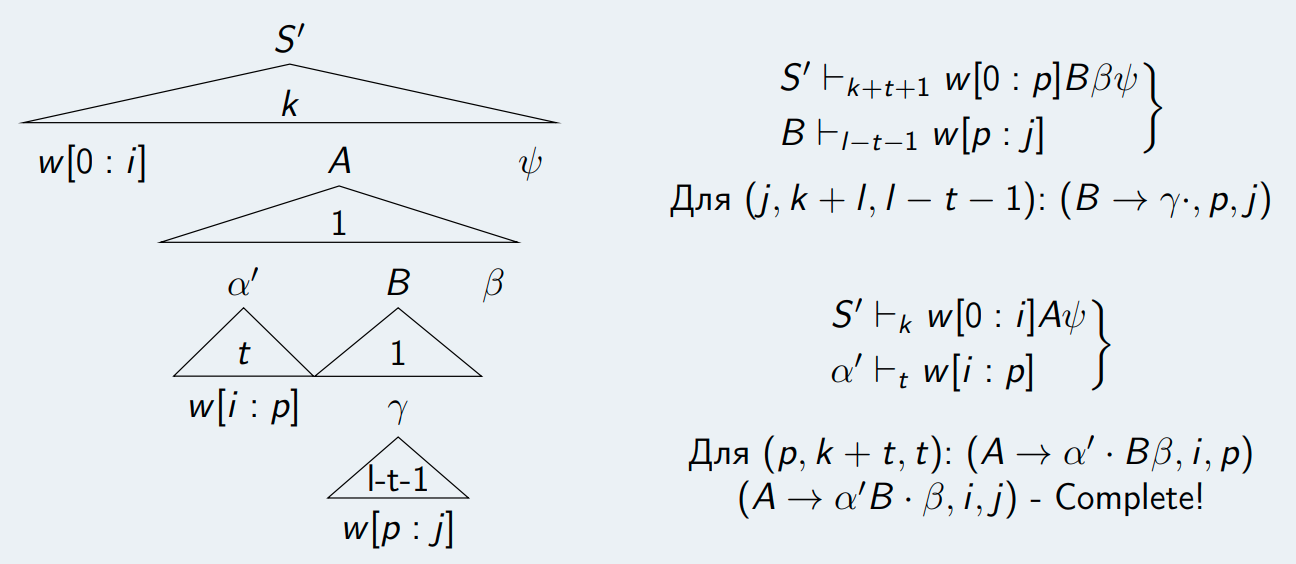
\includegraphics[scale=0.35]{assets/FullERli2.png}
		      \item $\alpha = \varepsilon$

		            \includegraphics[scale=0.4]{assets/FullERli3.png}
	      \end{enumerate}
\end{itemize}

\subsection{Оптимальный алгоритм и обоснование сложности}
\subsubsection*{Оптимальный алгоритм}
\begin{itemize}
	\item В $D_j$ надо быстро обращаться к правилам с $\cdot B$
	\item Храним в виде $D_j[B]$
	\item Правая часть -- в виде связного списка
	\item Быстрее -- вычислить id для каждой ситуации
	\item Меньше памяти -- вычислить hash для каждой ситуации
\end{itemize}

\subsubsection*{Обоснование сложности}
Пусть $\vert G\vert$ -- суммарное количество символов в правых частях правил.

\begin{itemize}
	\item Сложность Scan

	      Правила из $D_k[w[j]] \Rightarrow O(\vert D_j[w[j]]\vert) = O(\vert D_j\vert) = O(\vert w\vert\vert G\vert)$

	\item Сложность Predict

	      Перебираем правила $B \to \gamma$ -- $O(\vert P\vert)$. Рассматриваем $D_j[B]$ и помечаем, рассмотрена ли была ситуация с этим $B$.

	      Сложность для $D_j :\: O(\vert D_j\vert\vert P\vert) = O(\vert w\vert\vert G\vert^2)$
	\item Сложность Complete

	      Рассматриваем правила $(B \to \gamma\cdot,\, k) \in D_j$. Делаем перебор по $D_k[B] \Rightarrow$ количество обращений к $D_k :\: O(\vert D_0\vert + \vert D_1\vert + \cdots + \vert D_j\vert) = O(\vert w\vert^2\vert G\vert)$.

	      Количество правил $B \to \gamma:\: O(\vert G\vert) \Rightarrow$ асимптотика шага -- $O(\vert w\vert^2\vert G\vert^2)$
\end{itemize}

Количество шагов: $O(\vert w\vert)$

Итого на Scan: $O(\vert w\vert^2\vert G\vert)$

Итого на Predict: $O(\vert w\vert^2\vert G\vert^2)$

Итого на Complete: $O(\vert w\vert^3\vert G\vert^2)$

\subsection{Анализатор перенос-свёртка}
Смотри конспект Сорокина, который можно распечатать и принести на экзамен

\subsection{Операция перехода для LR-ситуаций}
Смотри конспект Сорокина, который можно распечатать и принести на экзамен

\subsection{Алгоритм построения LR-таблицы по LR-ситуациям}
Смотри конспект Сорокина, который можно распечатать и принести на экзамен

\subsection{Алгоритм разбора по LR-таблице}
Смотри конспект Сорокина, который можно распечатать и принести на экзамен

\subsection{ДМП-автоматы}
\begin{definition}
	Два перехода в МП-автомате: $\langle q_1,\, u_1,\, \alpha_1\rangle \to \langle q_1',\, \beta_1'\rangle$ и $\langle q_2,\, u_2,\, \alpha_2\rangle \to \langle q_2',\, \beta_2'\rangle$ называются \textbf{совместными}, если выполняются следующие условия:
	\begin{itemize}
		\item $q_1 = q_2$
		\item $u_1 \sqsubset u_2$ или $u_2 \sqsubseteq u_1$
		\item $\alpha_1 \sqsubseteq \alpha_2$ или $\alpha_2 \sqsubseteq \alpha_1$
	\end{itemize}
\end{definition}

\begin{definition}
	МП-автомат называется детерминированным, если в нём нет совместных переходов.
\end{definition}

\begin{definition}
	Пусть $M$ -- ДМП-автомат. Тогда языком, который задаёт данный автомат, называется
	\[
		L(M) = \{w \:\vert\: \exists q \in F :\: \langle q_0,\,w\$,\,\varepsilon\rangle\vdash\langle q,\,\varepsilon,\,\varepsilon\rangle\}
	\]
\end{definition}

\begin{lemma}
	Любой ДМП-автомат эквивалентен ДМП автомату с переходами
	\[
		\langle q_1,\,u,\,\alpha\rangle\to\langle q_2,\,\beta\rangle,\, \vert u\vert +\vert \alpha\vert \leq 1
	\]
\end{lemma}

\begin{proof}
	Разбиваем переходы совместно\dots
\end{proof}

\begin{theorem}
	Если $l$ -- длина самой длинной строки, которая может быть записана в ходе перехода в ДМП-автомате, то существует такая константа $N = F(\vert Q\vert,\, \vert \Gamma\vert,\, l)$ такая, что если $\langle q,\,\varepsilon,\, A\rangle \vdash_N\langle q',\,\varepsilon,\, \alpha\rangle,\, \vert \alpha\vert > 0$, то в ДМП-автомате возникнет цикл в конфигурации.
\end{theorem}

\begin{proof}
	Если длина стека в пути не больше $\vert Q\vert\vert\Gamma\vert l$, то в качестве $N$ возьмём
	\[
		N = \vert Q\vert(1 + \vert \Gamma\vert + \vert\Gamma\vert^2 +\cdots + \vert\Gamma\vert^{\vert Q\vert\vert\Gamma\vert l})
	\]
	где второй множитель обозначает максимальное число стеков длины $\leq \vert Q\vert\vert\Gamma\vert l$. Тогда по принципу дирихле найдётся одна конфигурация.

	Иначе
	\[
		\exists \langle q_0,\,\varepsilon,\,A\rangle\vdash_N\langle q',\,\varepsilon,\,\beta\rangle :\: \vert\beta\vert \geq \vert Q\vert\vert\Gamma\vert l + 1
	\]

	Давайте отмечать на нашем пути состояния так, чтобы длина стека у полученной подвыборки строго возрастала.

	Так как за переход длина стека меняется не более чем на $l$, то мы отметим хотя бы $\vert Q\vert\vert\Gamma\vert +1$ конфигураций.

	Тогда по принципу Дирихле $\exists$ два состояния:
	\[
		\langle q_1,\, \varepsilon,\, \alpha A\rangle,\,\langle q_1,\, \varepsilon,\, \alpha\gamma A\rangle
	\]
\end{proof}

\begin{theorem}
	Количество Shift'ов в LR-алгоритме ограничено сверху $\vert w\vert$, а количество Reduce'ов $\leq \vert w\vert\cdot N\cdot c$
\end{theorem}

\begin{proof}
	Введём потенциал, который является суммой:
	\begin{itemize}
		\item Числа терминальных символов грамматики на стеке
		\item Числа нетерминальных символов грамматики на стеке
		\item Удвоенного числа непрочитанных букв в слове
	\end{itemize}
	При Shift имеем +1 на стеке, но -2 непрочитанных букв.

	Отметим ситуации, после которых стек уменьшался -- после них потенциал уменьшается хотя бы на 1.

	Имея изначальный потенциал $2\vert w\vert$ и зная, что в конце он равен $0$, то получим, что количество ситуаций, разобранных выше, ограничено.

	Остаётся разобраться ситуации, когда Reduce не уменьшает стек, это происходит при обработке правил
	\[
		A \to \varepsilon ;\;\;\;\; A \to B
	\]
	Очевидно, таких правил ограниченное количество. Также, мы не можем прийти в соответствующую им ситуацию несколько раз, так как тогда мы зациклимся.
\end{proof}

\subsection{Приведение LR-алгоритма к распознаванию ДМП-автоматом}
\begin{proposition}
	Работа LR(1) алгоритма эмулируется работой ДМП-автомата.
\end{proposition}

\begin{proof}
	В качестве стека ДМП-автомата будем использовать стек LR-алгоритма (последовательность символ-вершина-\dots). То есть при операции Shift:
	\[
		\langle q_i,\, a,\, \varepsilon\rangle \to \langle \text{GOTO}(q_i,\, a),\, a\text{GOTO}(q_i,\, a)\rangle
	\]
	При операции Reduce снимаем со стека путь, переходим в соответствующую ситуацию из LR-таблицы и кладём на стек тот нетерминал, который считали.

	Почему этот автомат будет ДМП? Заметим, что свойство детерминированности эквивалентно отстутствию конфликтов, которых у нас нет по условию.
\end{proof}

\section{Конечные преобразователи}
\subsection{Конечные преобразователи и задаваемые ими преобразования}
\begin{definition}
	Конечным преобразователем (КПТелем) $M$ называется кортеж $M = \langle Q,\,\Sigma,\,\Gamma,\,\Delta,\, q_0,\, F\rangle$, где:
	\begin{itemize}
		\item $Q$ -- множество состояний, $\vert Q\vert < +\infty$
		\item $\Sigma$ -- входной алфавит, $\vert \Sigma\vert < +\infty$
		\item $\Gamma$ -- выходной алфавит, $\vert \Gamma\vert < +\infty$
		\item $\Delta \subset (Q \times \Sigma^*) \times (Q \times \Gamma^*)$ -- множество переходов
		\item $q_0$ -- стартовое состояние
		\item $F \subset Q$ -- множество завершающих состояний.
	\end{itemize}
\end{definition}

\begin{definition}
	\textbf{Конфигурацией КПтеля} $M$ называется тройка $\langle q,\,u,\,v\rangle \in Q \times \Sigma^* \times \Gamma^*$.

	Неформально:
	\begin{itemize}
		\item Находимся в состоянии $q$
		\item Осталось прочесть слово $u$
		\item Вывели слово $v$
	\end{itemize}
\end{definition}

\begin{definition}
	$\vdash$ -- наименьшее рефлексивное транзитивное отношение, что
	\[
		\forall \langle q_1,\,u\rangle \to\langle q_2,\, v\rangle \in \Delta
	\]
	выполнено:
	\[
		\forall y \in \Sigma^*,\, z \in \Gamma^* :\: \langle q_1,\, uv,\,z\rangle\vdash\langle q_2,\,y,\,zv\rangle
	\]
\end{definition}

\begin{definition}
	\textbf{Конечным преобразованием} будем называть
	\[
		\psi = \{(u,\,v) \in \Sigma^*\times\Gamma^* \:\vert\: \exists q \in F :\: \langle q_0,\,u,\,\varepsilon\rangle \vdash \langle q,\,\varepsilon,\,v\rangle\}
	\]
\end{definition}

\begin{proposition}
	Для любого КПтеля существует эквивалентный КПтель, для которого выполнено соотношение:
	\[
		\forall(\langle q_1,\,u\rangle\to\langle q_2,\, v\rangle) \in \Delta :\: \vert u\vert + \vert v\vert = 1
	\]
\end{proposition}

\begin{proof}
	\begin{enumerate}
		\item Раскроем все длинные переходы
		\item Удалим $\varepsilon:\varepsilon$ переходы по аналогии с НКА
	\end{enumerate}
\end{proof}

\begin{definition}
	Неудлиняющим гомоморфизмом $\psi$ называется  гомоморфизм, обладающим свойством
	\[
		\forall x \in \Sigma^* :\: \vert \psi(x)\vert \leq \vert x\vert
	\]
\end{definition}

\begin{theorem}
	Нива.

	Любое конечное преобразование можно представить в виде композиции:
	\begin{itemize}
		\item Обратного неудлиняющего гомоморфизма: $\phi^{-1}$
		\item Ограничения на регулярный язык $\text{id}_R$
		\item Неудлиняющего гомоморфизма: $\eta$
	\end{itemize}
\end{theorem}

\begin{proof}
	Пусть $\psi$ -- КП. Существует КПтель $M$ с 1-буквенными переходами.

	\begin{itemize}
		\item Промежуточный алфавит -- $\Delta$.
		\item Определим
		      \[
			      \phi(\langle q_1,\,u\rangle \to \langle q_2,\, v\rangle) = u;\;\;\;\;\eta(\langle q_1,\,u\rangle \to \langle q_2,\, v\rangle) = v
		      \]
		\item Тогда словами в нашем новом алфавите будут последовательности рёбер, по котором выводили в изначальном
		\item Заметим, что последовательности рёбер -- регулярный язык.
	\end{itemize}
\end{proof}

\subsection{Ограничение конечного преобразователя на регулярный вход}
\begin{theorem}
	Пусть $\psi :\: \Sigma^* \to \Gamma^*$ -- КП, $R$ -- регулярный язык. Тогда
	\[
		\psi\vert_R:\:R\to\Gamma^*
	\]
	является КП
\end{theorem}

\begin{proof}
	Пусть $T = \langle Q,\,\Sigma,\,\Gamma,\,\Delta_T,\, q_0,\, F_T\rangle$ -- КПтель: $\vert u\vert+\vert v\vert=1$ и $M = \langle P,\, \Sigma,\, \Delta_M,\, p_0,\, F_M\rangle$ -- ДКА: $L(M) = R$.

	Построим $T_M = \langle Q\times P,\, \Sigma,\, \Gamma,\, \Delta,\, (q_0,\, p_0),\, F_T\times F_M\rangle$, где $\Delta$ состоит из:
	\begin{itemize}
		\item $\langle(q_1,\,p_1),\, a\rangle\to\langle(q_2,\,p_2),\,\varepsilon\rangle$, если:
		      \begin{itemize}
			      \item $\langle q_1,\,a\rangle\to\langle q_2,\,\varepsilon\rangle\in\Delta_T$
			      \item $\langle p_1,\,a\rangle\to p_2 \in \Delta_M$
		      \end{itemize}
		\item $\langle(q_1,\,p),\,\varepsilon\rangle\to\langle(q_2,\,p),\,b\rangle$, если:
		      \begin{itemize}
			      \item $\langle q_1,\,\varepsilon\rangle\to\langle q_2,\,b\rangle\in\Delta_T$
		      \end{itemize}
	\end{itemize}
	Утверждается, что
	\[
		\langle(q_1,\,p_1),\,u,\,\varepsilon\rangle\vdash_{T_M}\langle q_2,\,\varepsilon,\,v\rangle \Leftrightarrow\begin{cases}
			\langle q_1,\,u,\,\varepsilon\rangle\vdash_T\langle q_2,\,\varepsilon,\,v\rangle \\
			\langle p_1,\,u\rangle\vdash_M\langle p_2,\,\varepsilon\rangle
		\end{cases}
	\]
	Докажем $\Rightarrow$ индукцией по длине вывода:
	\begin{itemize}
		\item База: 0 шагов
		      \begin{itemize}
			      \item $q_1 = q_2,\, p_1 = p_2,\, u = \varepsilon,\, v = \varepsilon$
			      \item $\langle q_1,\,u,\,\varepsilon\rangle\vdash_T\langle q_2,\,\varepsilon,\,v\rangle$
			      \item $\langle p_1,\,u\rangle\vdash_M\langle p_2,\,\varepsilon\rangle$
		      \end{itemize}
		\item Переход: $\langle(q_1,\,p_1),\,u,\,\varepsilon\rangle\vdash\langle(q_3,\,p_3),\,u_3,\,v_3\rangle\vdash_1\langle(q_2,\,p_2),\,\varepsilon,\,v\rangle$
		      \begin{itemize}
			      \item 1 случай: $u_3 = a$. Тогда $v_3 = v$
			      \item То есть $\langle q_3,\,a,\,\varepsilon\rangle\vdash_{T,\,1}\langle q_2,\,\varepsilon,\,\varepsilon\rangle,\,\langle p_3,\,a\rangle\vdash_{M,\,1}\langle p_2,\,\varepsilon\rangle$
			      \item Если $u = u'a$, то по предположению индукции: $\langle q_1,\,u',\,\varepsilon\rangle\vdash_T\langle q_3,\,\varepsilon,\,v\rangle,\,\langle p_1,\,u'\rangle\vdash_M\langle p_3,\,\varepsilon\rangle$
			      \item Воспользовавшись транзитивностью, получим требуемое:
			            \begin{align*}
				            \langle q_1,\,u'a,\,\varepsilon\rangle\vdash_T\langle q_3,\,a,\,v\rangle\vdash_{T,\,1}\langle q_2,\,\varepsilon,\,v\rangle \\
				            \langle p_1,\,u'a\rangle\vdash_M\langle p_3,\,a\rangle\vdash_{M,\,1}\langle p_2,\,\varepsilon\rangle
			            \end{align*}
			      \item 2 случай: $u_3 = \varepsilon,\,v = v_3b,\, p_2 = p_3$
			      \item $\langle q_3,\,\varepsilon,\,\varepsilon\rangle\vdash_{T,\,1}\langle q_2,\,\varepsilon,\,b\rangle$
			      \item Пользуемся транзитивностью:
			            \begin{align*}
				            \langle q_1,\,u,\,\varepsilon\rangle\vdash_T\langle q_3,\,\varepsilon,\,v_3\rangle\vdash_{T,\,1}\langle q_2,\,\varepsilon,\, v_3b\rangle \\
				            \langle p_1,\,u\rangle\vdash_M\langle p_3,\,\varepsilon\rangle=\langle p_2,\,\varepsilon\rangle
			            \end{align*}
		      \end{itemize}
	\end{itemize}
	В обратную сторону $\Leftarrow$ индукцией по сумме длин вывода в $T$ и $M$:
	\begin{itemize}
		\item База: вывод суммарно за 0 шагов
		      \begin{itemize}
			      \item $q_1 = q_2,\, p_1 = p_2$
			      \item $u = \varepsilon$, так как $M$ -- ДКА, $v = \varepsilon$
			      \item По рефлексивности
			            \[
				            \langle(q_1,\,p_1),\,u,\,\varepsilon\rangle\vdash_{T_M}\langle(q_2,\,p_2),\,\varepsilon,\,v\rangle
			            \]
		      \end{itemize}
		\item Переход: $\langle q_1,\,u,\,\varepsilon\rangle\vdash_T\langle q_3,\,u_3,\,v_3\rangle\vdash_{T,\,1}\langle q_2,\,\varepsilon,\,v\rangle$
		      \begin{itemize}
			      \item 1 случай: $\langle q_3,\,a\rangle\to\langle q_2,\,\varepsilon\rangle$
			      \item Тогда: $u_3 = a,\, v_3 = v,\, u = u'a$
			      \item Тогда найдётся $p_4 :\: \langle p_1,\,u'a\rangle\vdash_T\langle p_4,\,a\rangle\vdash_{T,\,1}\langle p_2,\,\varepsilon\rangle$
			      \item $\langle q_1,\,u',\,\varepsilon\rangle\vdash_T\langle q_3,\,\varepsilon,\,v\rangle$
			      \item Воспользуемся предположением $\langle(q_1,\,p_1),\,u',\,\varepsilon\rangle\vdash_{T_M}\langle(q_3,\,p_4),\,\varepsilon,\,v\rangle$:
			            \[
				            \langle(q_1,\,p_1),\,u'a,\,\varepsilon\rangle\vdash_{T_M}\langle(q_3,\,p_4),\,a,\,v\rangle\vdash_{T_M,\,1}\langle(q_2,\,p_2),\,\varepsilon,\,v\rangle
			            \]
			      \item 2 случай: $\langle q_1,\,\varepsilon\rangle\to\langle q_2,\,b\rangle$
			      \item Тогда $u_3 = \varepsilon,\, v = v_3b$
			      \item Предположение индукции: $\langle(q_1,\,p_1),\,u,\,\varepsilon\rangle\vdash_{T_M}\langle(q_3,\,p_2),\,\varepsilon,\,v_3\rangle$
			      \item Воспользуемся транзитивностью:
			            \[
				            \langle(q_1,\,p_1),\,u,\,\varepsilon\rangle\vdash_{T_M}\langle(q_3,\,p_2),\,\varepsilon,\,v_3\rangle \vdash_{T_M,\,1}\langle(q_2,\,p_2),\,\varepsilon,\,v_3b\rangle
			            \]
		      \end{itemize}
	\end{itemize}
	Теперь зная данное прекрасное свойство, докажем теорему:
	\begin{itemize}
		\item $(u,\,v) \in \psi_{T_M}$
		\item $\exists q \in F_T,\, p \in F_M :\: \langle(q_0,\,p_0),\,u,\,\varepsilon\rangle\vdash\langle(q,\,p),\,\varepsilon,\,v\rangle$
		\item $\exists q \in F_T,\, p \in F_M :\: \langle q_0,\,u,\,\varepsilon\rangle\vdash\langle q,\,\varepsilon,\,v\rangle,\,\langle p_0,\,u\rangle\vdash\langle p,\,\varepsilon\rangle$
		\item $(u,\,v) \in \psi_T,\, u \in R$
		\item $(u,\, v) \in \psi\vert_R$
	\end{itemize}
\end{proof}

\subsection{Замкнутость конечных преобразований относительно композиции}
\begin{theorem}
	Пусть $\psi_1 :\: \Sigma^* \to \Gamma^*$ и $\psi_2 :\: \Gamma^* \to \Pi^*$ -- КП. Тогда $\psi_2\circ\psi_1 :\: \Sigma^* \to \Pi^*$ -- КП.
\end{theorem}

\begin{proof}
	Пусть $\psi_1 = \psi_1(M_1):\: M_1 = \langle Q,\,\Sigma,\,\Gamma,\,\Delta_1,\,q_0,\,F_1\rangle$ и $\psi_2 = \psi_2(M_2) :\: M_2 = \langle P,\, \Gamma,\, \Pi,\, \Delta_2,\, p_0,\, F_2\rangle$.

	Тогда построим преобразователь-композицию
	\[
		M := \langle Q\times P,\, \Sigma,\, \Pi,\, \Delta,\, (q_0,\, p_0),\, F_1\times F_2\rangle
	\]
	где $\Delta$ состоит из:
	\begin{itemize}
		\item $\langle(q_1,\,p),\,a\rangle\to\langle(q_2,\,p),\,\varepsilon\rangle$, если $\langle q_1,\,a\rangle \to \langle q_2,\,\varepsilon\rangle \in \Delta_1$
		\item $\langle(q_1,\,p_1),\,\varepsilon\rangle\to\langle(q_2,\,p_2),\,\varepsilon\rangle$, если:
		      \begin{itemize}
			      \item $\langle q_1,\,\varepsilon \rangle\to\langle q_2,\,b\rangle \in \Delta_1$
			      \item $\langle p_1,\,b\rangle\to\langle p_2,\,\varepsilon\rangle \in \Delta_2$
			      \item $\langle(q,\,p_1),\,\varepsilon\rangle\to\langle(q,\,p_2),\,c\rangle$, если $\langle p_1,\,\varepsilon\rangle\to\langle p_2,\,c\rangle \in \Delta_2$
		      \end{itemize}
	\end{itemize}
	Утверждается, что
	\[
		\langle(q_1,\,p_1),\,u,\,\varepsilon\rangle\vdash_M\langle(q_2,\,p_2),\,\varepsilon,\,v\rangle\Leftrightarrow \exists z \in \Gamma^* :\: \begin{cases}
			\langle q_1,\,u,\,\varepsilon\rangle\vdash_{M_1}\langle q_2,\,\varepsilon,\,z\rangle \\
			\langle p_1,\,z,\,\varepsilon\rangle\vdash_{M_2}\langle p_2,\,\varepsilon,\, v\rangle
		\end{cases}
	\]
	В начале докажем $\Rightarrow$ индукцией по длине вывода:
	\begin{itemize}
		\item База 0 шагов: $q_1 = q_2,\, p_1 = p_2,\, u = \varepsilon,\, v = \varepsilon$
		      \begin{itemize}
			      \item $z := \varepsilon$
			      \item $\langle q_1,\,u,\,\varepsilon\rangle\vdash_{M_1}\langle q_2,\,\varepsilon,\,\varepsilon\rangle$
			      \item $\langle p_1,\,\varepsilon,\,\varepsilon\rangle\vdash_{M_2}\langle p_2,\,\varepsilon,\,v\rangle$
		      \end{itemize}
		\item Переход: читаем букву $a$:
		      \begin{itemize}
			      \item $\langle q_1,\,a\rangle\to\langle q_3,\,\varepsilon\rangle\in\Delta_{M_1}$
			      \item $\langle(q_1,\,p_1),\,au',\,\varepsilon\rangle\vdash_1\langle(q_3,\,p_1),\,u',\,\varepsilon\rangle\vdash\langle(q_2,\,p_2),\,\varepsilon,\,v\rangle$
			      \item По предположению $\exists z :\: \langle q_3,\,u',\,\varepsilon\rangle\vdash_{M_1}\langle q_2,\,\varepsilon,\,z\rangle$ и $\langle p_1,\,z,\,\varepsilon\rangle\vdash_{M_2}\langle p_2,\,\varepsilon,\,v\rangle$
			      \item Объединив, получим
			            \[
				            \langle q_1,\,au',\,\varepsilon\rangle\vdash_{M_1,\,1}\langle q_3,\,u',\,\varepsilon\rangle\vdash_{M_1}\langle q_2,\,\varepsilon,\,z\rangle
			            \]
		      \end{itemize}

		\item Переход: пишем букву $c$:
		      \begin{itemize}
			      \item $\langle p_1,\,\varepsilon\rangle \to \langle p_3,\,c\rangle \in \Delta_{M_2}$
			      \item $\langle(q_1,\,p_1),\,u,\,\varepsilon\rangle\vdash_{M_2,\,1}\langle(q_1,\,p_3),\,u,\,c\rangle\vdash\langle(q_2,\,p_2),\,\varepsilon,\,cv'\rangle$
			      \item По предположению $\exists z :\: \langle q_1,\,u,\,\varepsilon\rangle\vdash_{M_1}\langle q_2,\,\varepsilon,\,z\rangle,\,\langle p_3,\,z,\,\varepsilon\rangle\vdash_{M_2}\langle p_2,\,\varepsilon,\,v'\rangle$
			      \item Объединяем по транзитивности
			            \[
				            \langle p_1,\,z,\,\varepsilon\rangle\vdash_{M_2,\,1}\langle p_3,\,z,\,c\rangle\vdash_{M_2}\langle p_2,\,\varepsilon,\,cv'\rangle
			            \]
		      \end{itemize}
		\item Переход: делаем $\varepsilon:\:\varepsilon$ переход
		      \begin{itemize}
			      \item По определению такого перехода, $\exists x :\: \langle q_1,\,\varepsilon,\,\varepsilon\rangle\vdash_{M_1,\,1}\langle q_3,\,\varepsilon,\,x\rangle,\, \langle p_1,\,x,\,\varepsilon\rangle\vdash_{M_2,\,1}\langle p_3,\,\varepsilon,\,\varepsilon\rangle$
			      \item $\langle(q_1,\,p_1),\,u,\,\varepsilon\rangle\vdash_{M,\,1}\langle(q_3,\,p_3),\,u,\,\varepsilon\rangle\vdash\langle(q_2,\,p_2),\,\varepsilon,\,v\rangle$
			      \item По предположению $\exists z :\: \langle q_3,\,u,\,\varepsilon\rangle\vdash\langle q_2,\,\varepsilon,\,z\rangle,\, \langle p_3,\,z,\,\varepsilon\rangle\vdash_{M_2}\langle p_2,\,\varepsilon,\,v\rangle$
			      \item Объединив всё, что знаем
						\begin{align*}
							\langle q_1,\,u,\,\varepsilon\rangle\vdash_{M_1,\,1}\langle q_3,\,u,\,x\rangle\vdash_{M_1}\langle q_2,\,\varepsilon,\,xz\rangle\\
							\langle p_1,\,xz,\,\varepsilon\rangle_{M_2,\,1}\langle p_3,\,z,\,\varepsilon\rangle\vdash_{M_2}\langle p_2,\,\varepsilon,\,v\rangle
						\end{align*}
					\end{itemize}
	\end{itemize}
	В $\Leftarrow$ докажем индукцией по сумме длин вывода из $M_1$ и $M_2$.
	\begin{itemize}
		\item База: 0 шагов
		\begin{itemize}
			\item Тогда $u = \varepsilon,\, v = \varepsilon,\, z = \varepsilon$
			\item $q_1 = q_2,\, p_1 = p_2$
		\end{itemize}
		\item Переход: читаем букву $a$ из $u$:
		\begin{itemize}
			\item $\langle q_1,\,au',\,\varepsilon\rangle\vdash_{M_1,\,1}\langle q_3,\,u',\,\varepsilon\rangle\vdash_{M_1}\langle q_2,\,\varepsilon,\,z\rangle$
			\item Предположение $\langle(q_3,\,p_1),\,u',\,\varepsilon\rangle \vdash \langle(q_2,\,p_2),\,\varepsilon,\,v\rangle$
			\item Тогда
			\[
				\langle(q_1,\,p_1),\,au',\,\varepsilon\rangle\vdash_1\langle(q_3,\,p_1),\,u',\,\varepsilon\rangle
			\]
		\end{itemize}
		\item Переход: пишем букву $c$ из $v$:
		\begin{itemize}
			\item $\langle p_1,\,z,\,\varepsilon\rangle\vdash_{M_2,\,1}\langle p_3,\,z,\,c\rangle\vdash_{M_2}\langle p_2,\,\varepsilon,\,cv'\rangle$
			\item Предположение $\langle(q_1,\,p_3),\,u,\,\varepsilon\rangle\vdash\langle(q_2,\,p_2),\,\varepsilon,\,v'\rangle$
			\item Тогда
			\[
				\langle(q_1,\,p_1),\,u,\,\varepsilon\rangle\vdash_1\langle(q_1,\,p_3),\,u,\,c\rangle\vdash\langle(q_2,\,p_2),\,\varepsilon,\,cv'\rangle
			\]
		\end{itemize}
		\item Переход: пишем $b$ в $z$ и читаем из $z$:
		\begin{itemize}
			\item По условию $\langle q_1,\,u,\,\varepsilon\rangle\vdash_{M_1,\,1}\langle q_3,\,u,\,b\rangle\vdash_{M_1}\langle q_2,\,\varepsilon,\, bz'\rangle$ и $\langle p_1,\,bz',\,\varepsilon\rangle\vdash_{M_2,\,1}\langle p_3,\,z',\,\varepsilon\rangle\vdash_{M_2}\langle p_2,\,\varepsilon,\,v\rangle$
			\item По предположению индукции: $\langle(q_3,\,p_3),\,u,\,\varepsilon\rangle\vdash\langle(q_2,\,p_2),\,\varepsilon,\,v\rangle$
			\item Тогда 
			\[
				\langle(q_1,\,p_1),\,u,\,\varepsilon\rangle\vdash_M\langle(q_3,\,p_3),\,u,\,\varepsilon\rangle
			\]
		\end{itemize}
	\end{itemize}
	Теперь, зная это прекрасное свойство, докажем теорему:
	\begin{itemize}
		\item $(u,\, v) \in \psi(M)$
		\item $\exists q \in F_1,\, p \in F_2 :\: \langle(p_0,\,q_0),\,u,\,\varepsilon\rangle\vdash\langle(q,\,p),\,\varepsilon,\,v\rangle$
		\item $\exists q \in F_1,\, p \in F_2,\, z \in \Gamma^*$:
		\begin{align*}
			\langle q_0,\,u,\,\varepsilon\rangle\vdash_{M_1}\langle q,\,\varepsilon,\,z\rangle\\
			\langle p_0,\,z,\,\varepsilon\rangle\vdash_{M_2}\langle p,\,\varepsilon,\,v\rangle
		\end{align*}
		\item $\exists z \in \Gamma^* :\: (u,\,z) \in \psi_1,\, (z,\, v) \in \psi_2$
		\item $(u,\,v) \in \psi_2\circ\psi_1$
	\end{itemize}
\end{proof}

\end{document}